\documentclass[11pt]{beamer}

\usetheme{metropolis}

\usepackage{graphicx}
\usepackage{physics}
\usepackage{adjustbox}
\usepackage{caption}
\usepackage{chemformula}
\usepackage{quoting}
\usepackage[style=chem-angew,backend=bibtex]{biblatex}
\bibliography{references}
%
% Choose how your presentation looks.
%
% For more themes, color themes and font themes, see:
% http://deic.uab.es/~iblanes/beamer_gallery/index_by_theme.html
%
\mode<presentation>
{
  \usetheme{default}      % or try Darmstadt, Madrid, Warsaw, ...
  \usecolortheme{default} % or try albatross, beaver, crane, ...
  \usefonttheme{default}  % or try serif, structurebold, ...
  \setbeamertemplate{navigation symbols}{}
  \setbeamertemplate{caption}[numbered]
  \setbeamerfont{footnote}{size=\tiny}
} 

\usepackage[english]{babel}
\usepackage[utf8]{inputenc}
\graphicspath{{../lectureMW/image/}}

\AtBeginSection[]{
\begin{frame}{Outline}
  \tableofcontents[currentsection]
\end{frame}
}

\title{Chapter 1+2: Matter, Atoms, Ions, and Periodic Table}
\institute{Chemistry Department, Cypress College}
\date{August 30, 2022}

\begin{document}

\begin{frame}
  \titlepage
\end{frame}

\begin{frame}{Class Announcements}
  \begin{itemize}
  \item Delayed homework assignment 1
  \item File submissions - merge all into one file (preferred)
  \item Office Hour: M 11:30am - 12:30pm in Science, Engineering,
    and Mathematics (SEM) building in Room 150
  \item First canvas quiz this Friday at 11am due next Tues
    at 11:59pm
%  \item Attend my co-instructor Prof. Lenore Landis:
%    M 12:45-2:15 PM in SEM 312, TTh 1:25-2:10 PM in SEM 314, W 12:45-3:15 PM
%    in SEM 312 or SEM 161
  \end{itemize}
\end{frame}

\begin{frame}{Lecture Weekly Agenda}
  \begin{itemize}
  \item Cover Ch 1 - pg $1 - 55$
  \item Go over Ch 2 - pg $56 - 88$
  \item In-class Ch 1+2 worksheet
  \end{itemize}
\end{frame}

\begin{frame}{One More Time: Sig Figs}
  Perform the calculation and write the appropriate number
  of significant figures
  
  \begin{equation*}
    \frac{1.0\times 10^{-2}\text{g} - 1.2\times 10^{-3}\text{g}}
    {1.579\times 10^{-1}\text{cm}}
  \end{equation*}
\end{frame}

\begin{frame}{One More Time: Unit Conversion}
  Convert the following.

  \begin{itemize}
  \item 2.9 nm to dam
  \item 3 hHz to mHz
  \end{itemize}
\end{frame}

\section{Chapter 1}

\subsection{Matter and Its Classification}

\begin{frame}{Chemistry Connection: Climate Change}
  \centering
  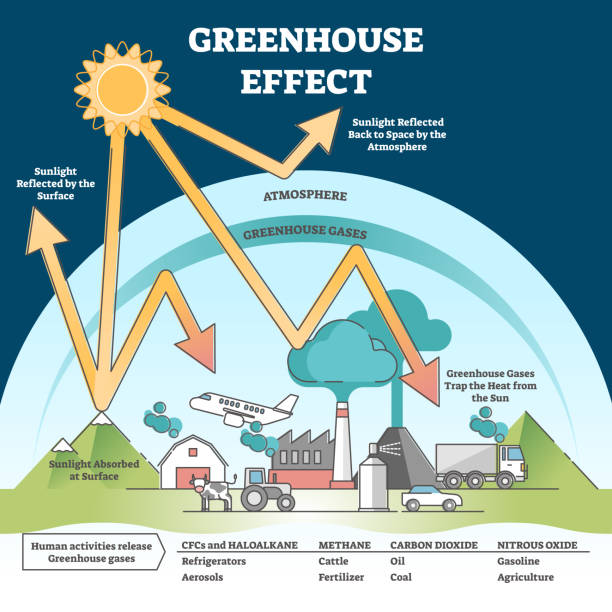
\includegraphics[scale=1.5]{greenhouse_effect}
\end{frame}

\begin{frame}{Conservation of Mass}
  Any system closed to all transfers of matter and energy, the mass
  of the system must remain constant over time
\end{frame}

\begin{frame}{Photosynthesis: Converting H$_2$O and CO$_2$ into Sugar}
  \centering
  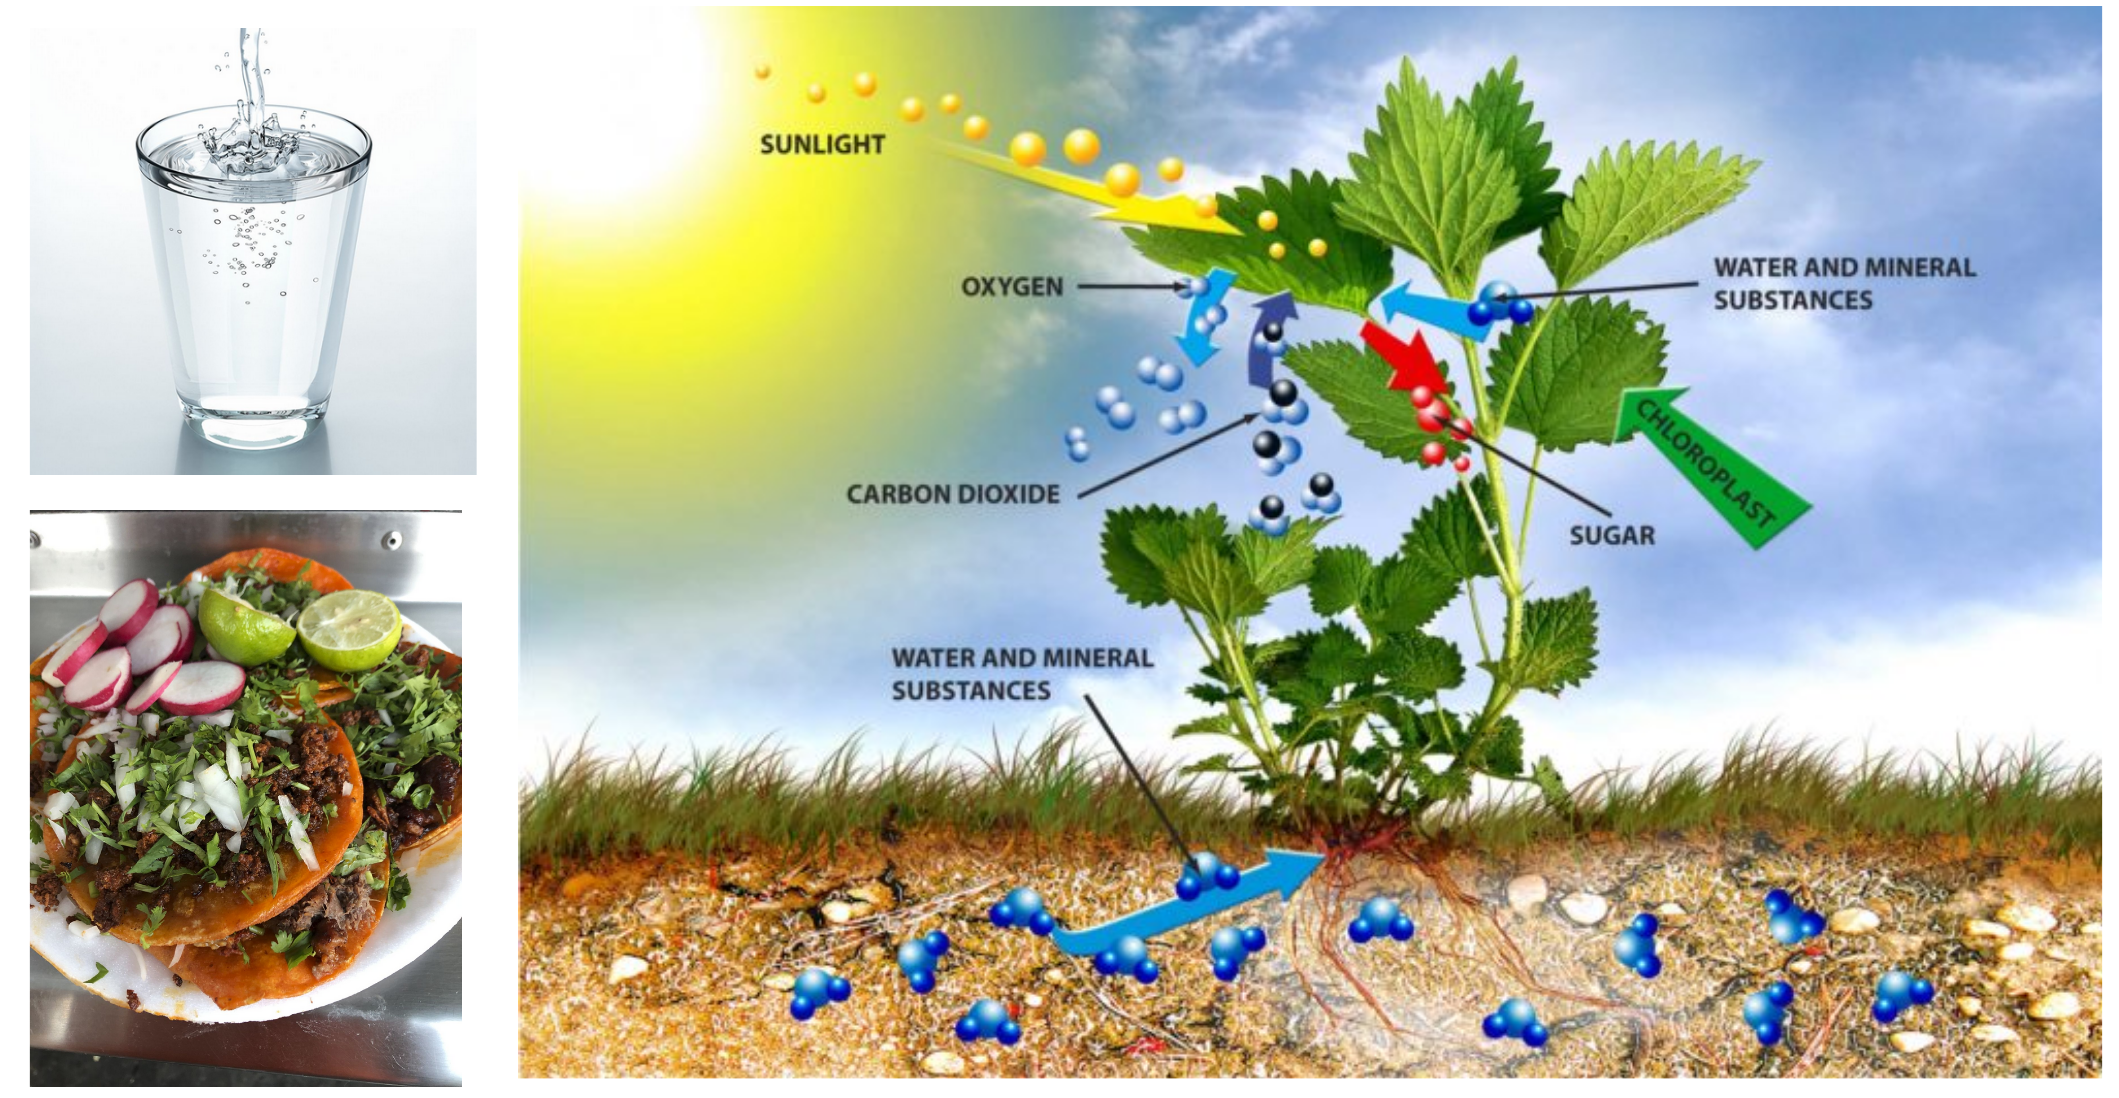
\includegraphics[trim={8in 0 0 0},clip,width=1\linewidth]{food_pic}
\end{frame}

\begin{frame}{Combustion Reaction}
  \centering
  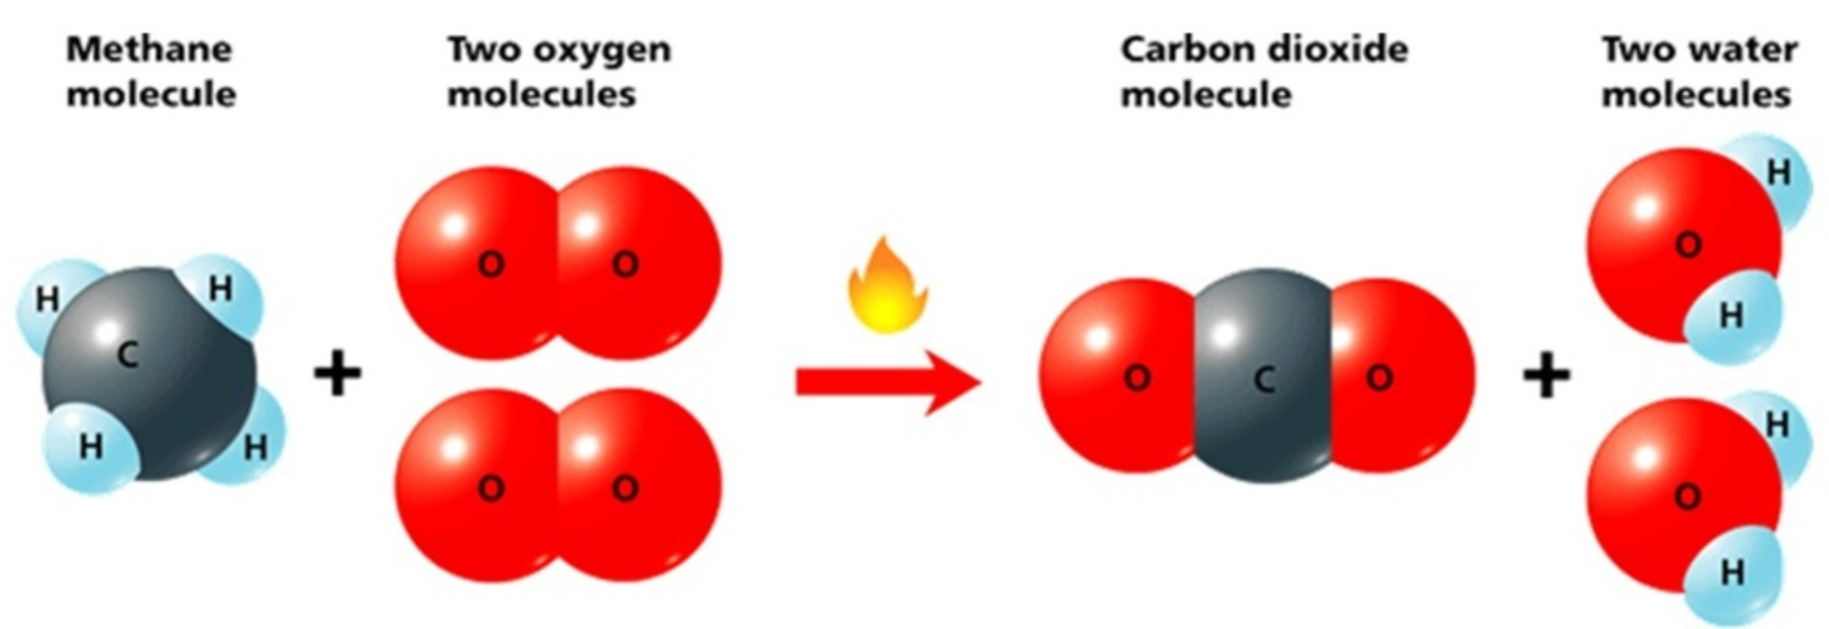
\includegraphics[scale=0.175]{methane_burn}
\end{frame}

\begin{frame}{Classification: Composition of Matter}
  \textbf{Pure substance} - cannot be separated into components

  \textbf{Mixture} - consists at least 2 pure substances mixed
  together
\end{frame}

\begin{frame}{Classification: Composition of Matter}
  \textbf{Pure substance} - cannot be separated into components
  
  Checkout the preiodic table (\href{https://ptable.com}{ptable})
  
  \centering
  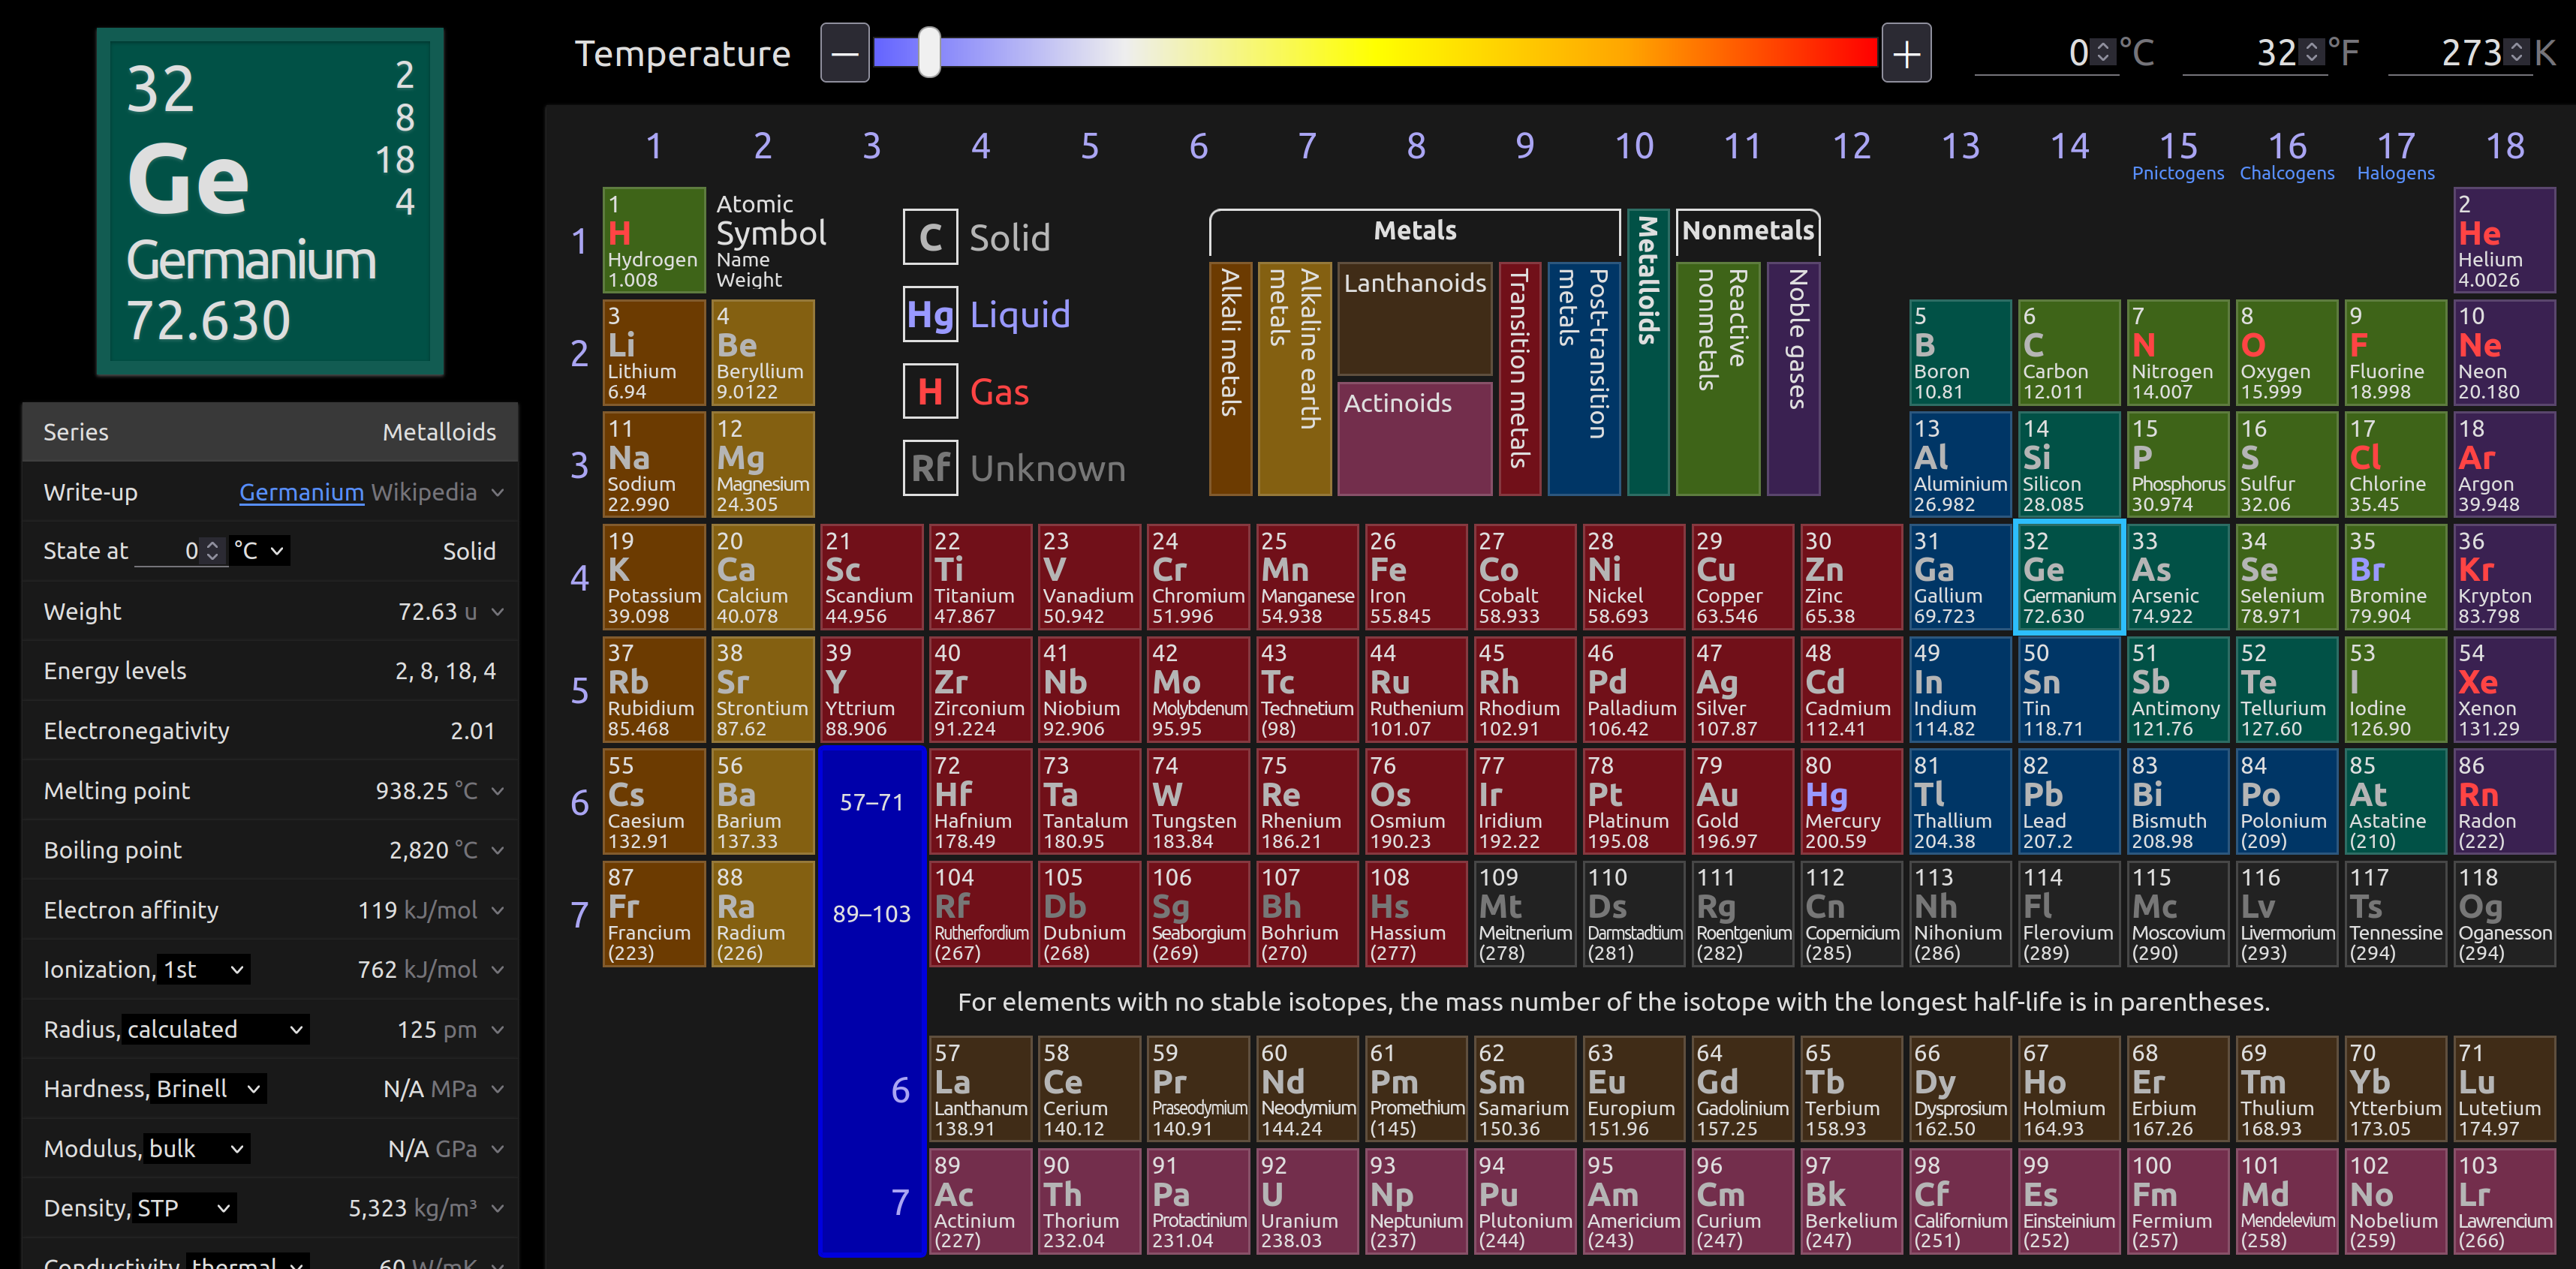
\includegraphics[width=\linewidth]{ptable}
\end{frame}

\begin{frame}{Examples of Pure Substances}
  \centering
  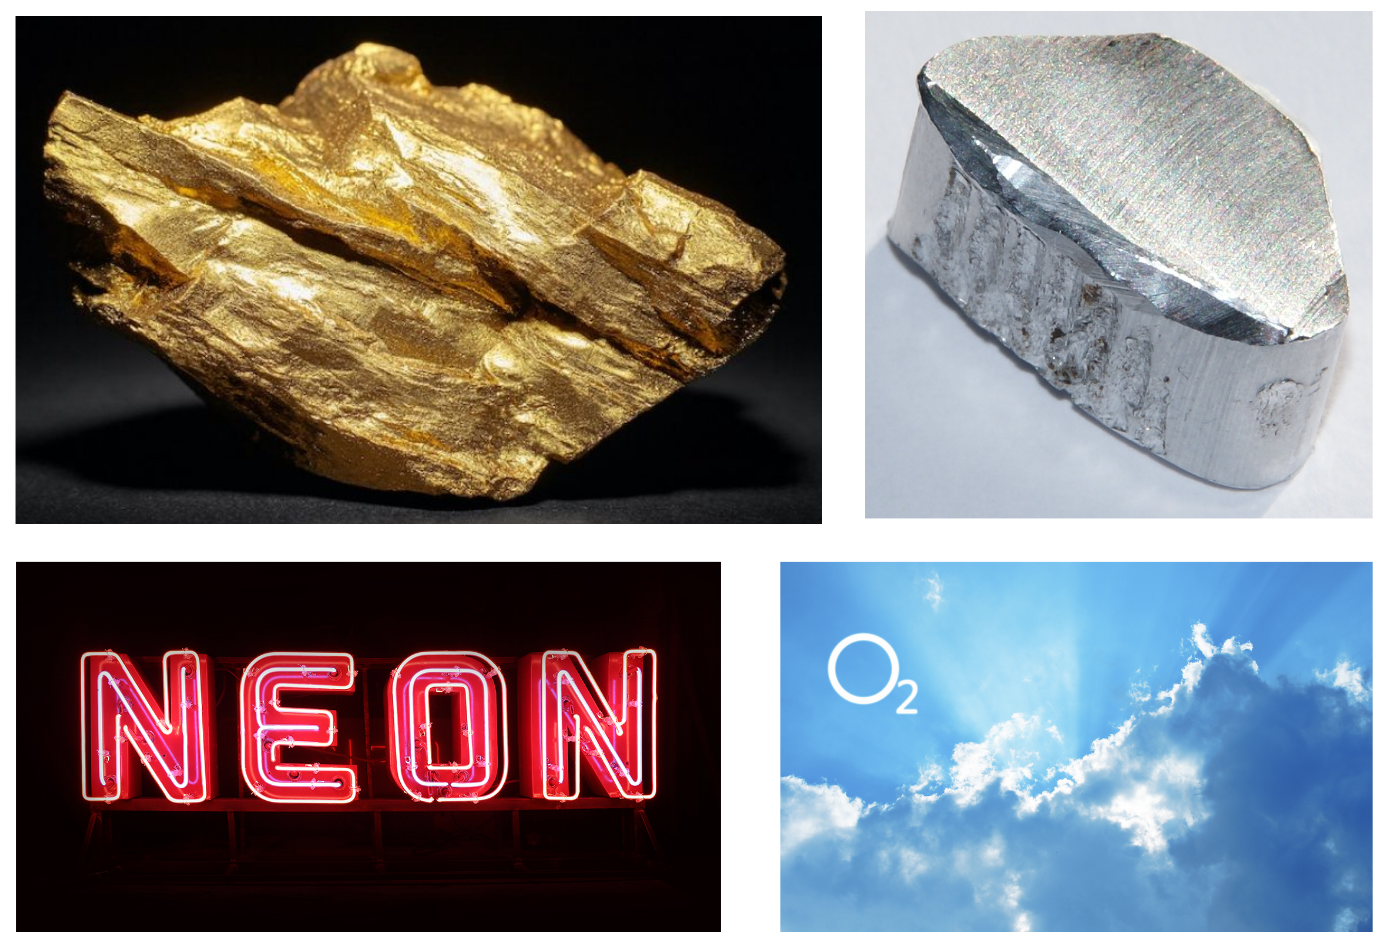
\includegraphics[width=\linewidth]{pure}
\end{frame}

\begin{frame}{Is water a pure substance?}
  \centering
  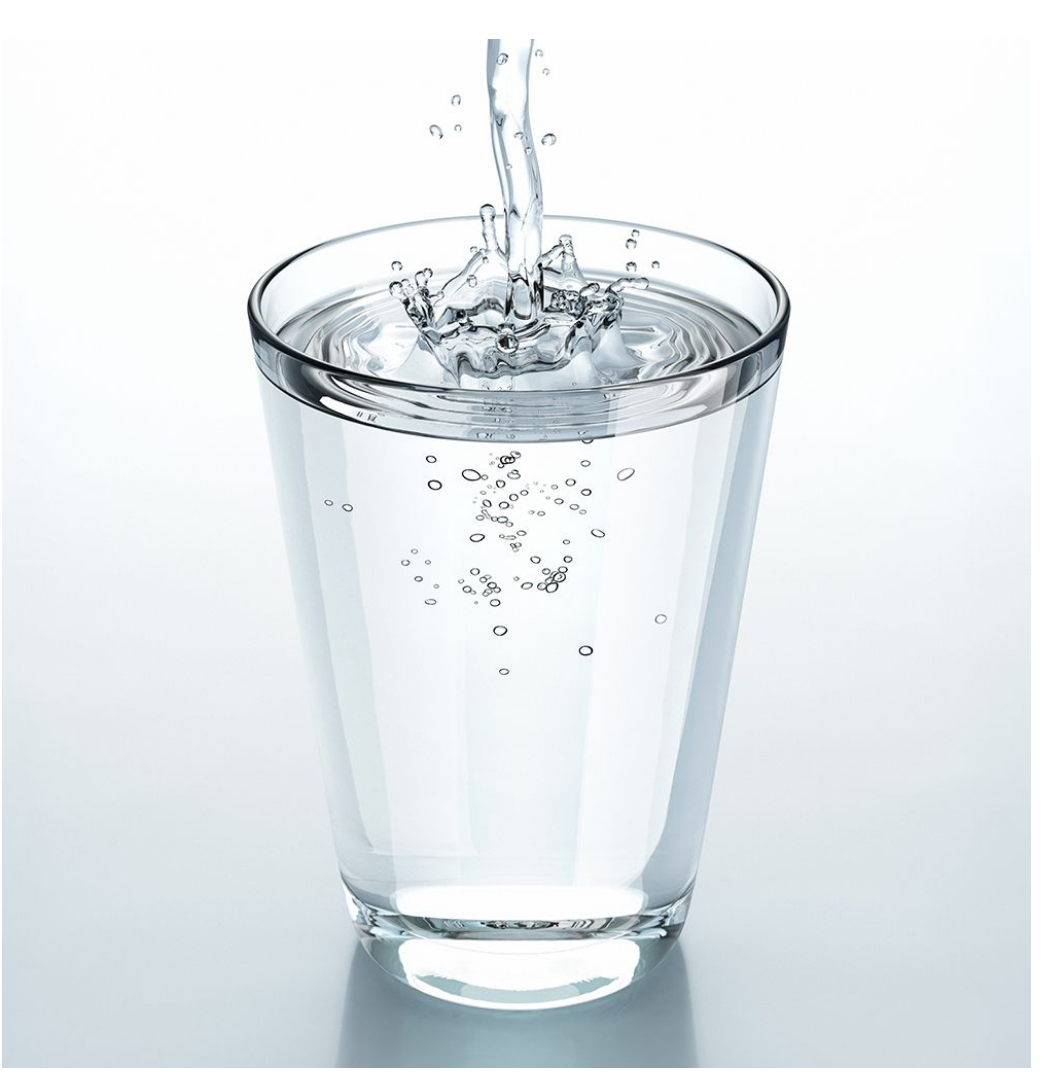
\includegraphics[scale=0.2]{water}
\end{frame}

\begin{frame}{Types of Mixtures}
  \centering
  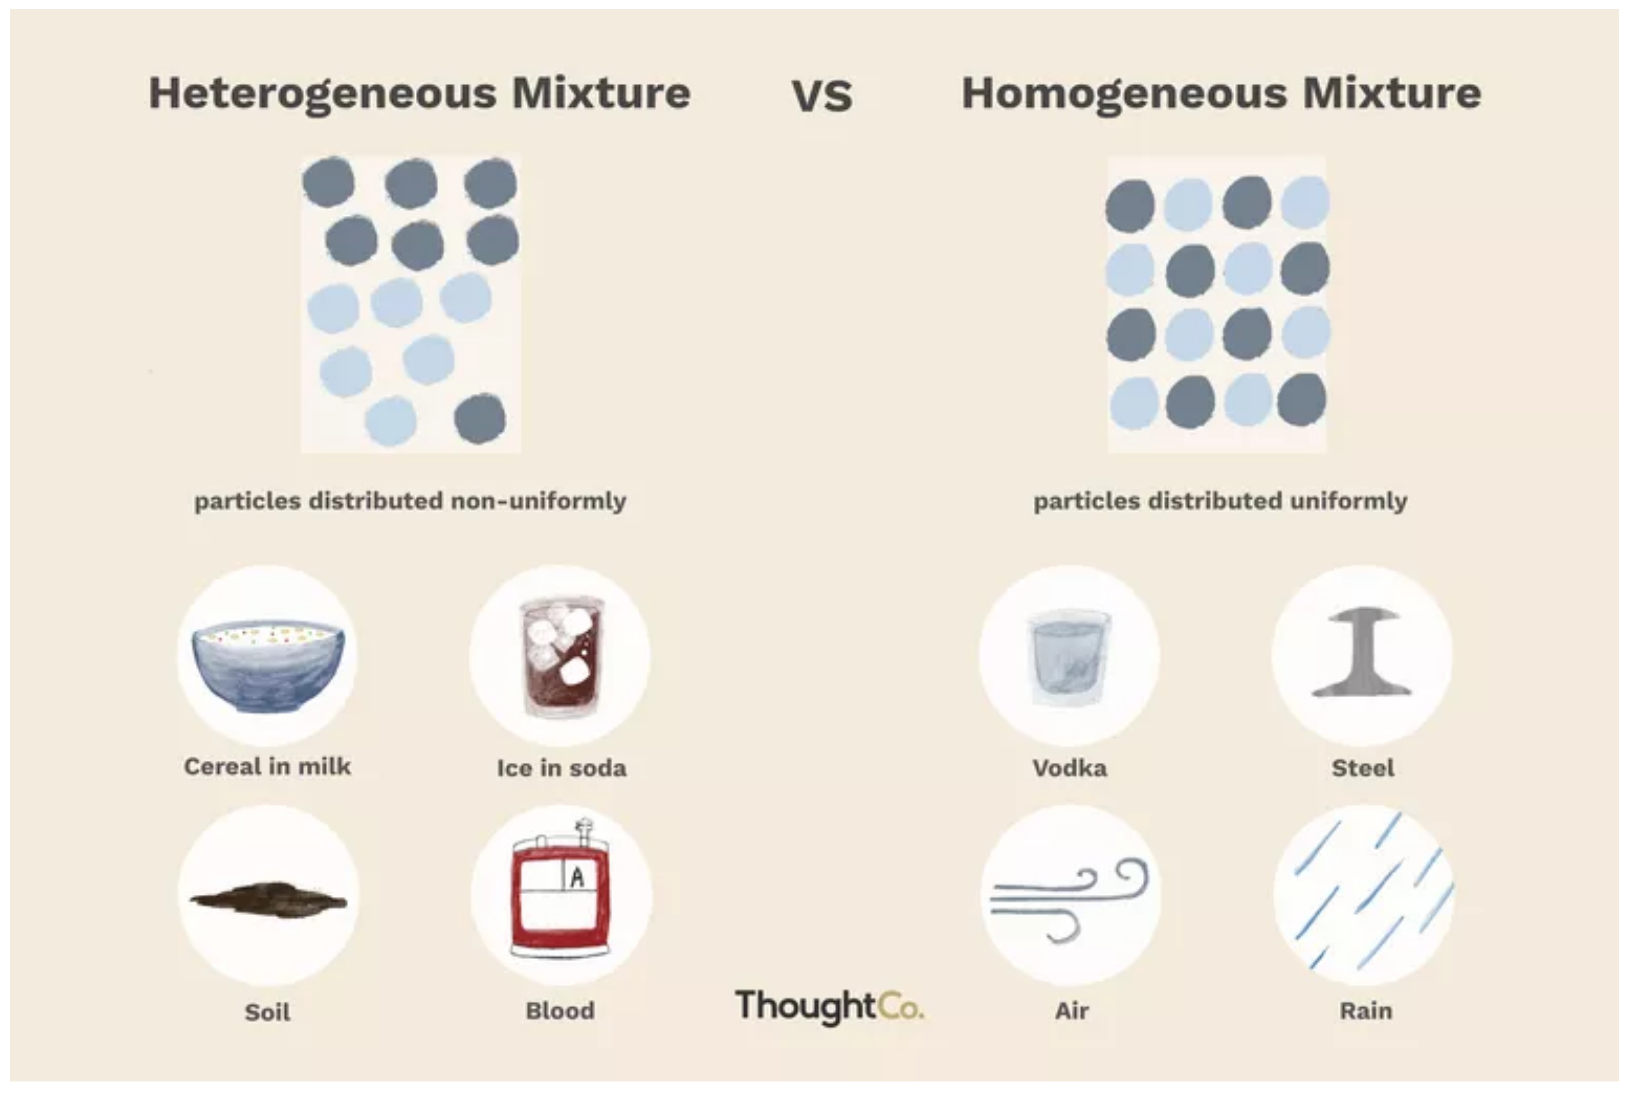
\includegraphics[width=\linewidth]{mixtures}
\end{frame}

\begin{frame}{States of Matter: Water}
  \centering
  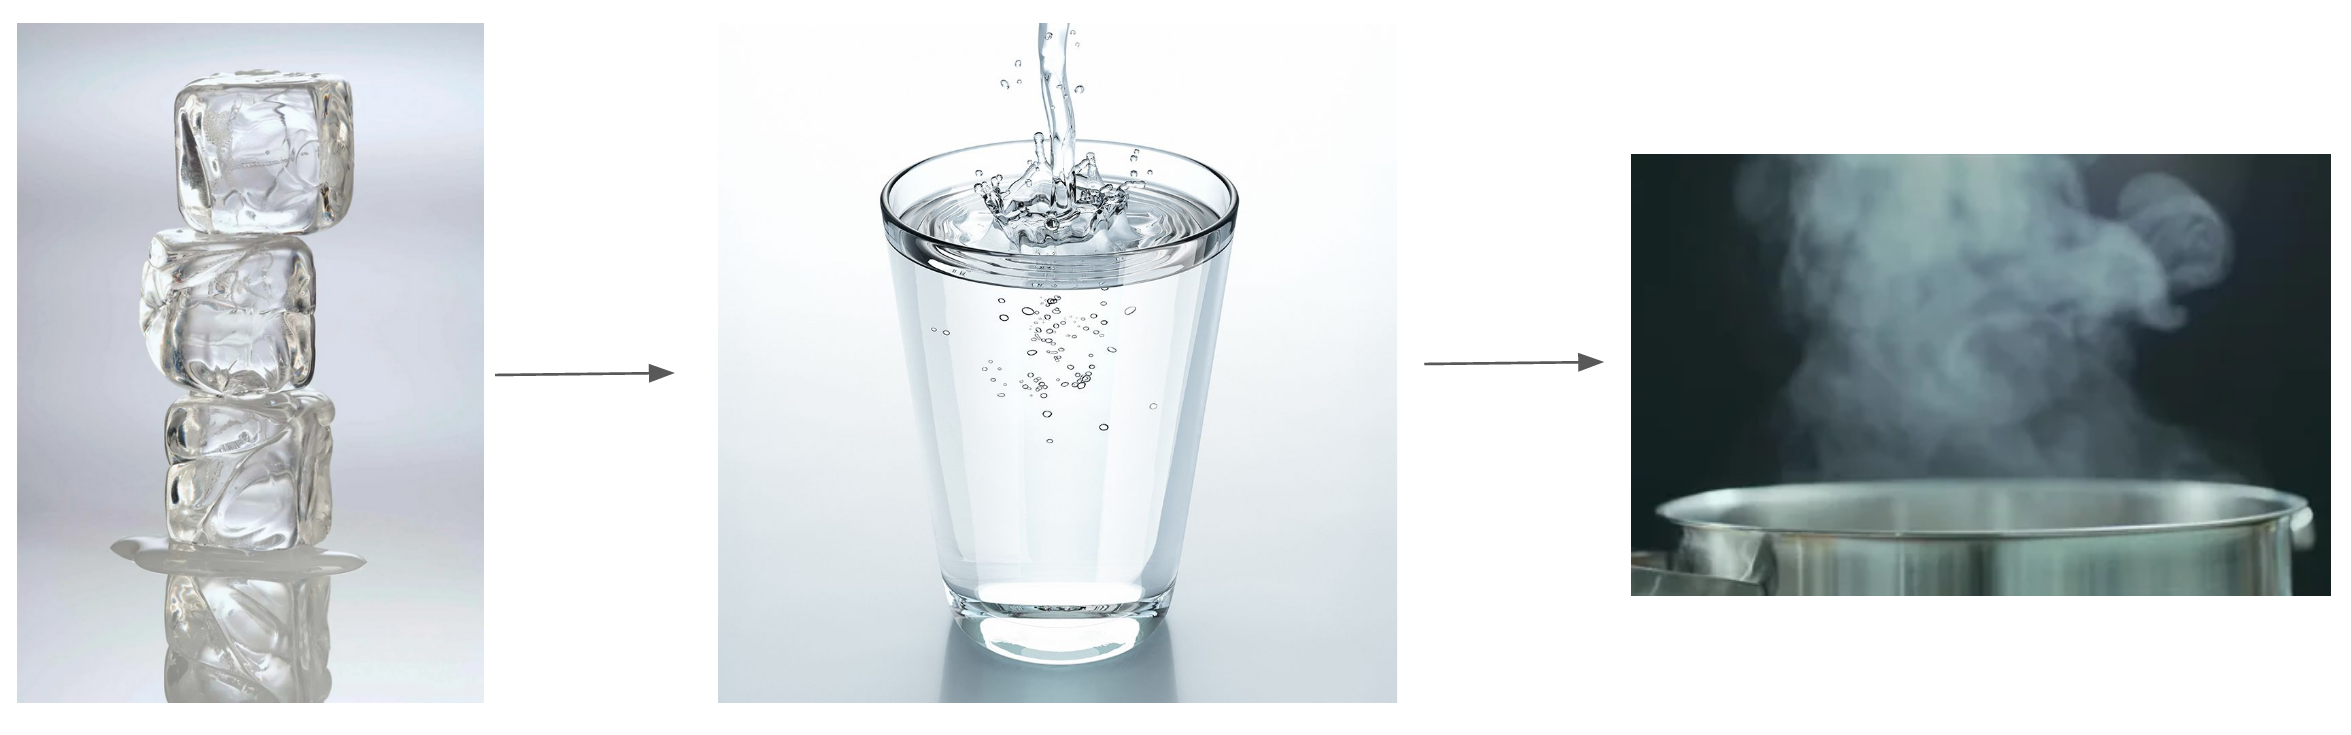
\includegraphics[width=\linewidth]{water_states}
  \vspace{-0.2in}
  \begin{itemize}
  \item Solid has the smallest volume whereas gas occupies
    the largest space
  \item Water molecules have the most energy in which state?
  \item Notation for states - H$_2$O(s), H$_2$O(l), H$_2$O(g)
  \item \textbf{Aqueous state} - substance dissolved in water
    e.g. NaCl(aq)
  \end{itemize}
\end{frame}

\subsection{Chemical and Physical Changes}

\begin{frame}{Physical Properties}
  A characteristic that can be observed or measured without
  changing the composition of a substance
  
  \centering
  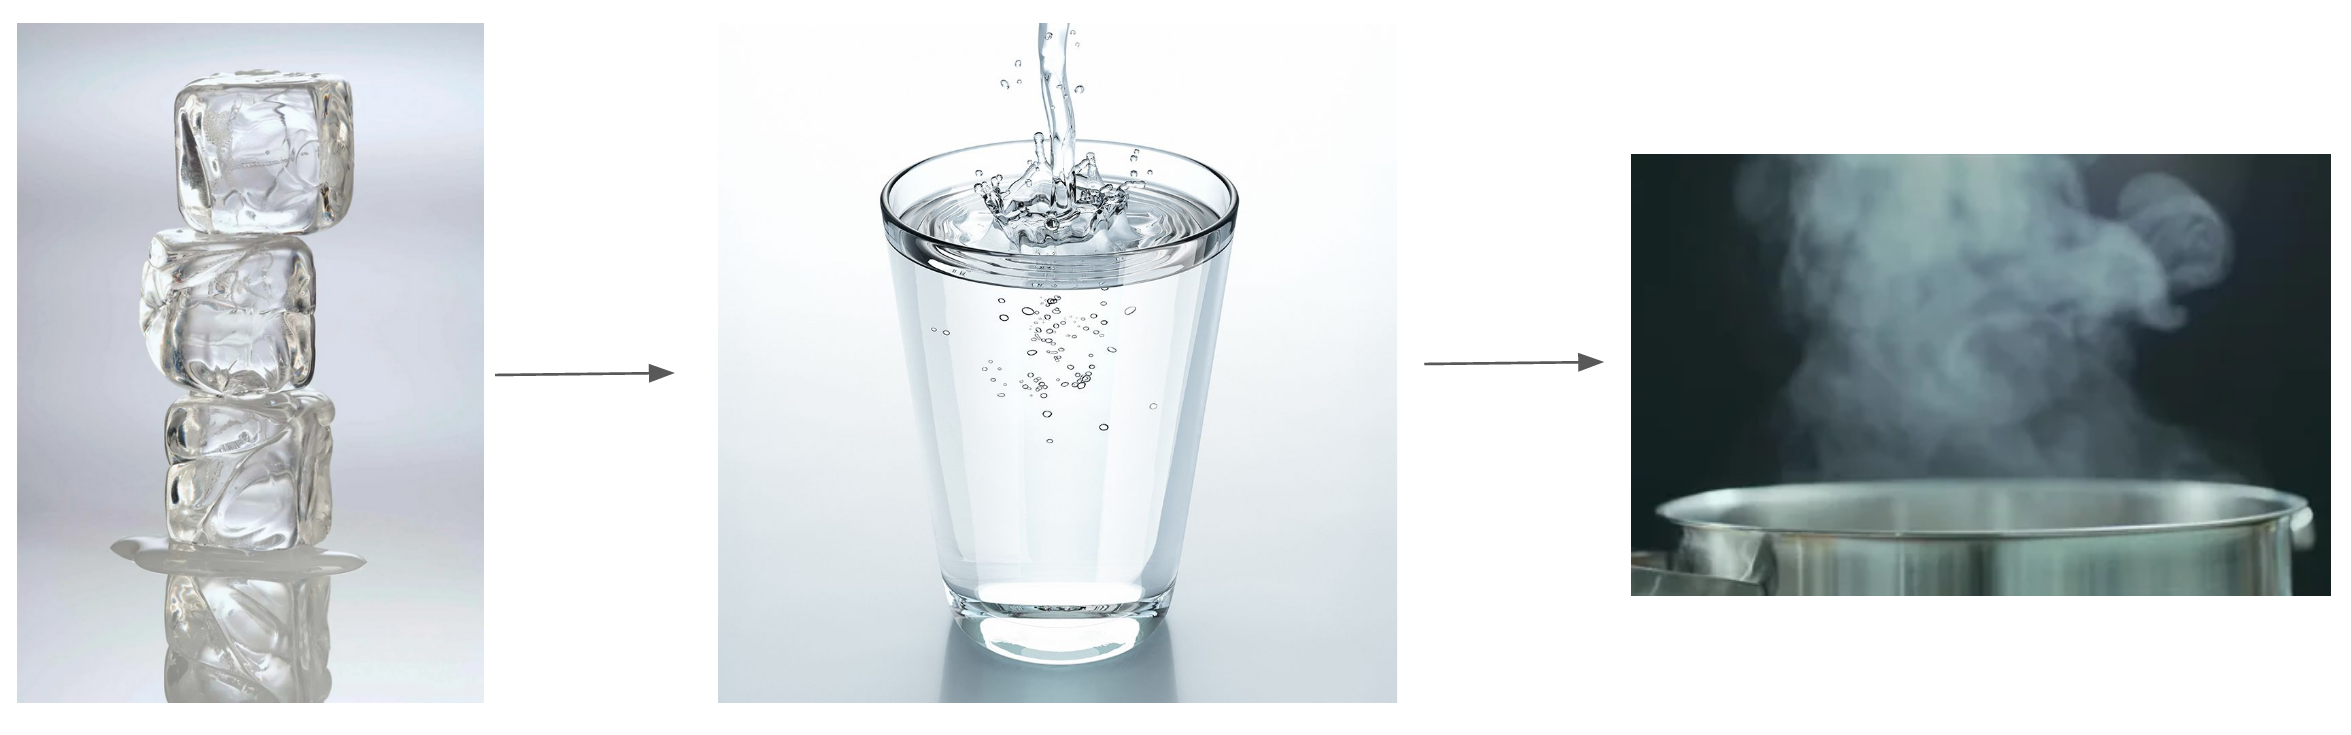
\includegraphics[width=\linewidth]{water_states}
\end{frame}

\begin{frame}{Quantifying Physical Properties}
  \begin{itemize}
  \item Mass - quantifies matter; measuring in grams
  \item Volume - amount of space occupied; measuring in L
  \item Density - ratio of mass and volume
  \end{itemize}
  \centering
  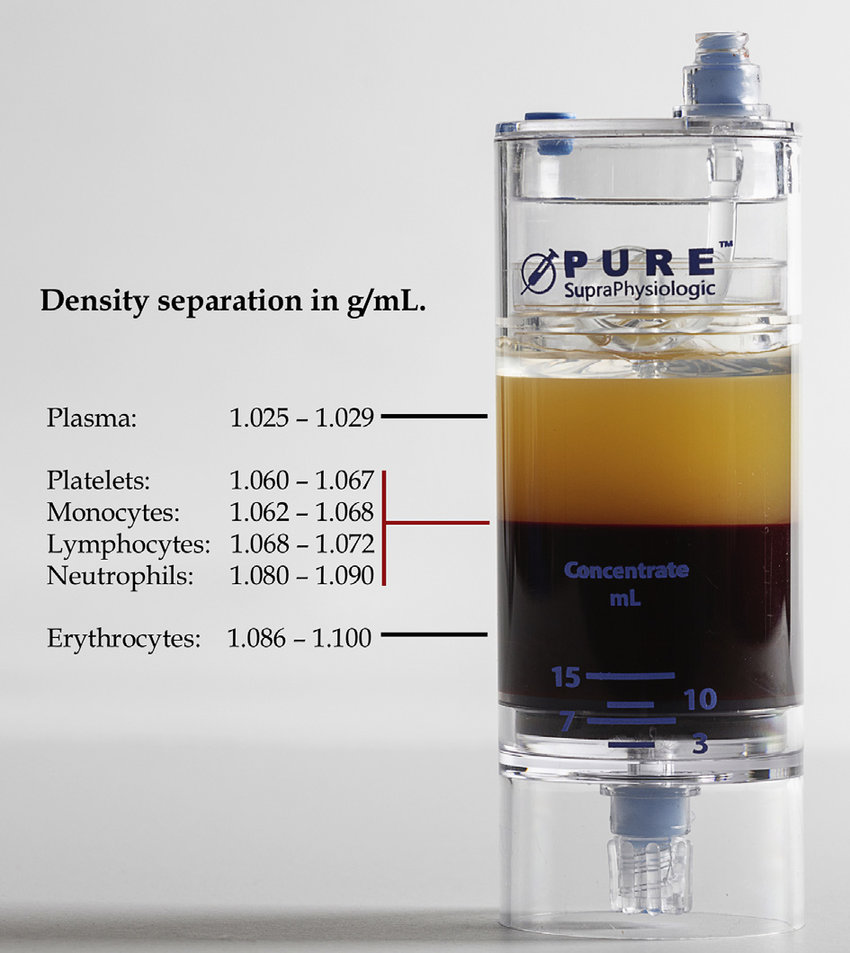
\includegraphics[scale=0.14]{dens_liquids}
  \begin{itemize}
  \item Temperature - quantifies the intensity of heat in a substance
    or object
  \end{itemize}
\end{frame}

\begin{frame}{Chemical Properties}
  A characteristic of a particular subtance that can be observed
  in a chemical reaction e.g. combustion

  \centering
  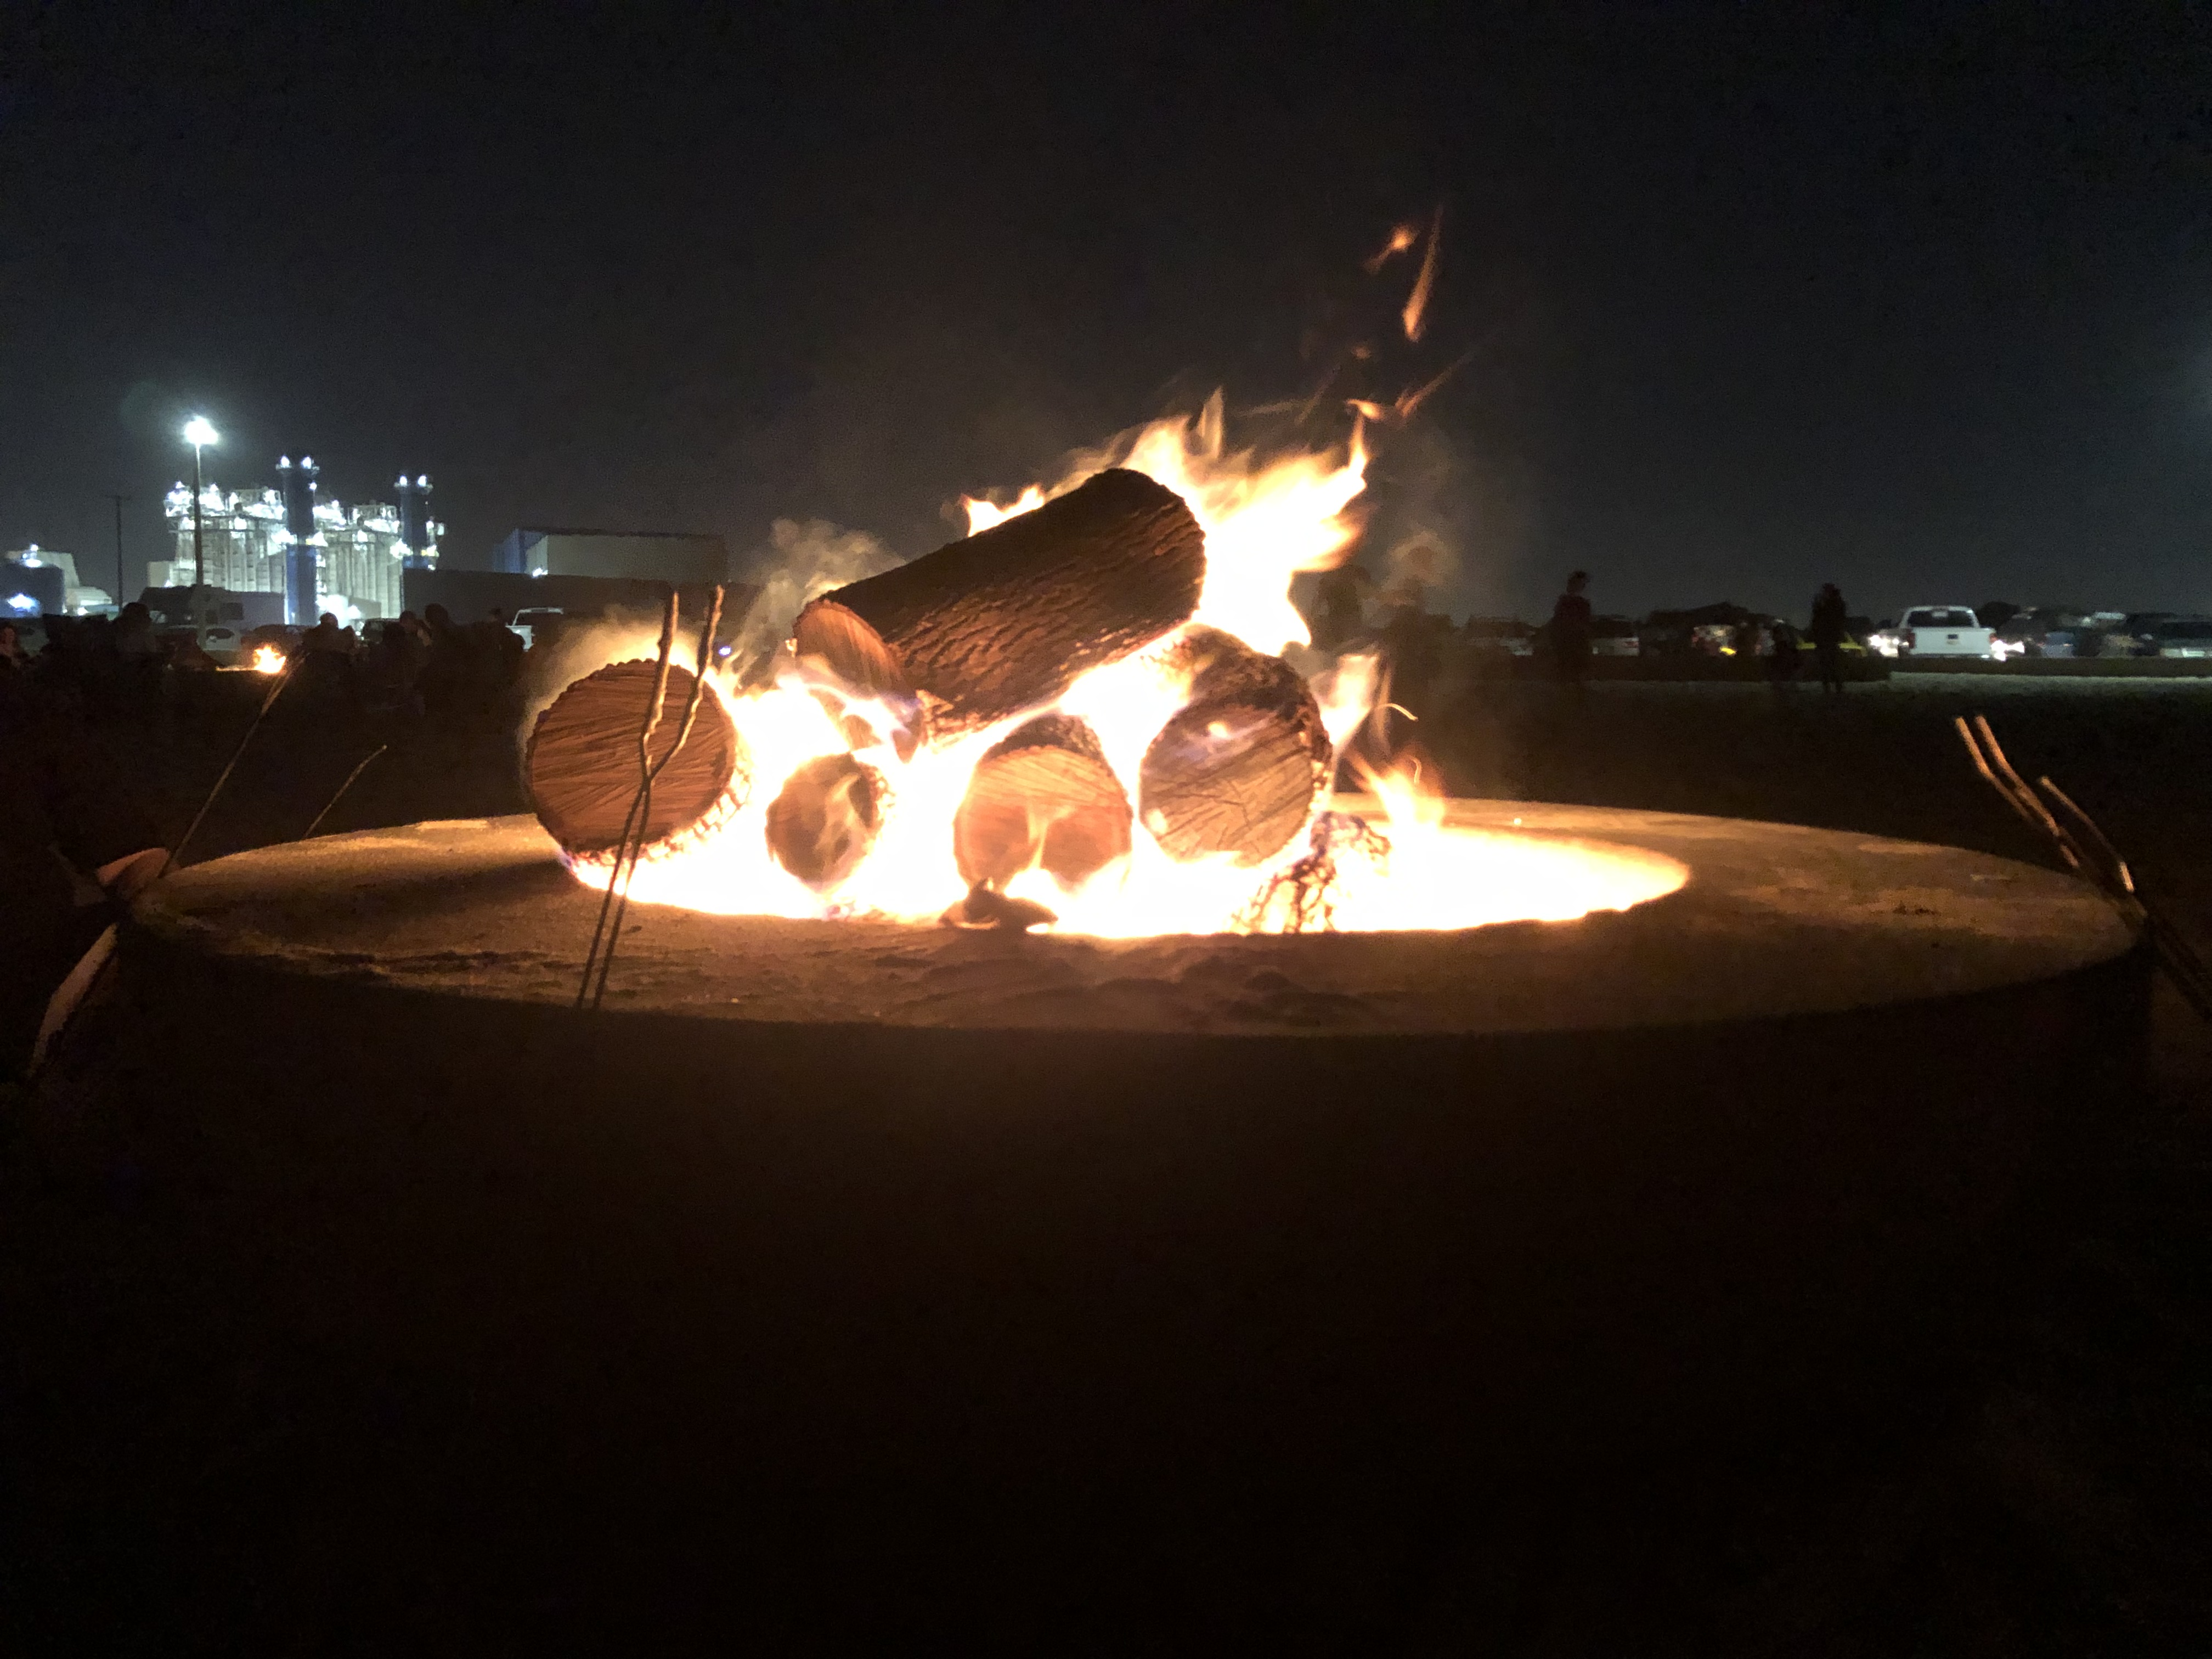
\includegraphics[scale=0.05]{bonfire}
\end{frame}

\begin{frame}{Practice: Classify the following as chemical or physical changes}
  \begin{enumerate}
  \item Melting solid gold into liquid gold
  \item Combining copper and tin to form bronze (an alloy)
  \item Electrolysis of water (H$_2$O) into hydrogen (H$_2$) gas and oxygen (O$_2$)
    gas
  \item Filtering algae from water
  \end{enumerate}
\end{frame}

\subsection{Potential and Kinetic Energy}

\begin{frame}{Potential vs Kinetic Energy}
  \textbf{Potential Energy} - Stored energy; elastic, chemical, and
  gravitational

  \textbf{Kinetic Energy} - Involves motion

  \vfill
\end{frame}

\subsection{Scientific Method}

\begin{frame}{Research Uses Scientific Method}
  \begin{enumerate}
  \item Gather observations
  \item Ask a question. Propose a hypothesis
    which is a supposed explanation of a given phenomenon
  \item Design and perform your experiment
  \item If results support the hypothesis, then propose
    a theory, which explains the observation. If not, then revise
    the hypothesis.
  \end{enumerate}
\end{frame}

\begin{frame}{Everyday Life Example: Failure to Toast}
  \centering
  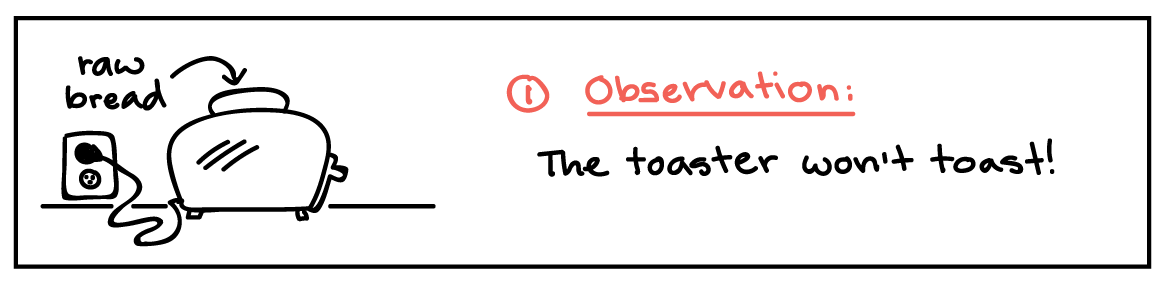
\includegraphics[scale=1]{fail_toast}
\end{frame}

\begin{frame}{Hypothesis - Ask the Question}
  \centering
  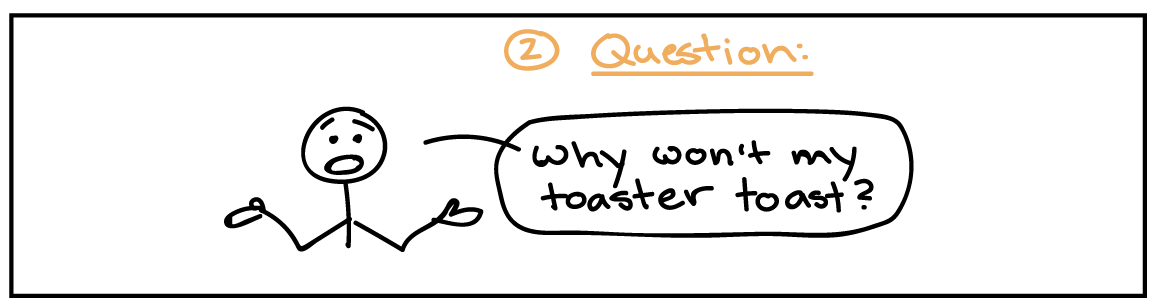
\includegraphics[scale=1]{toast_q}
\end{frame}

\begin{frame}{Propose Hypothesis}
  \centering
  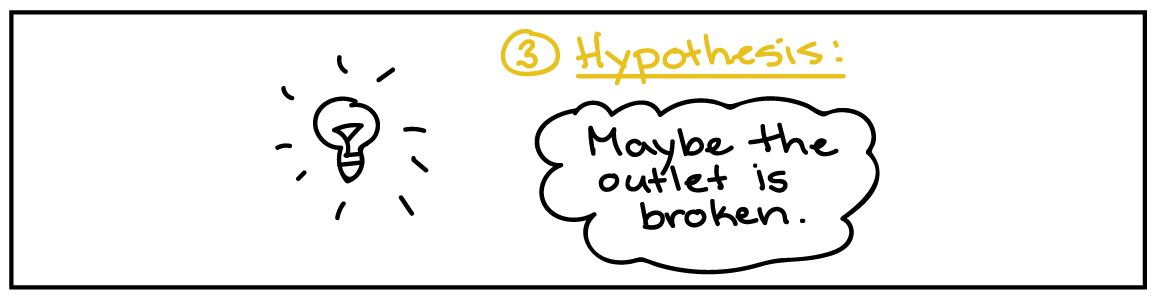
\includegraphics[scale=1]{toast_hypoth}
\end{frame}

\begin{frame}{Make a Prediction}
  \centering
  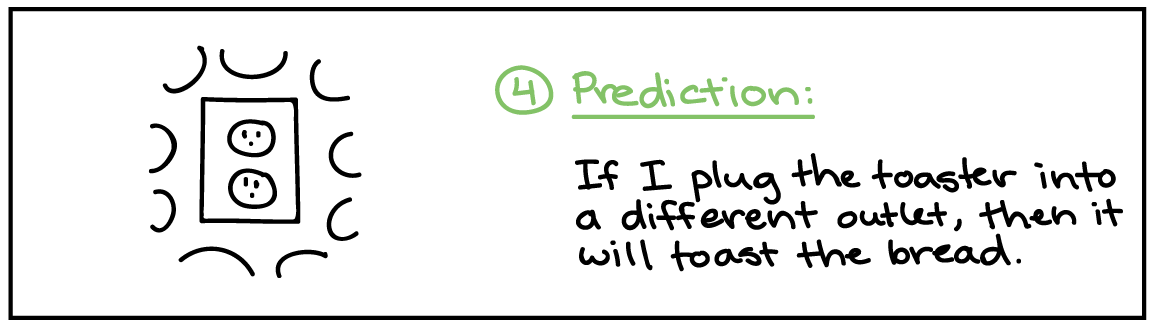
\includegraphics[scale=1]{toast_predict}
\end{frame}

\begin{frame}{Test the Prediction}
  \centering
  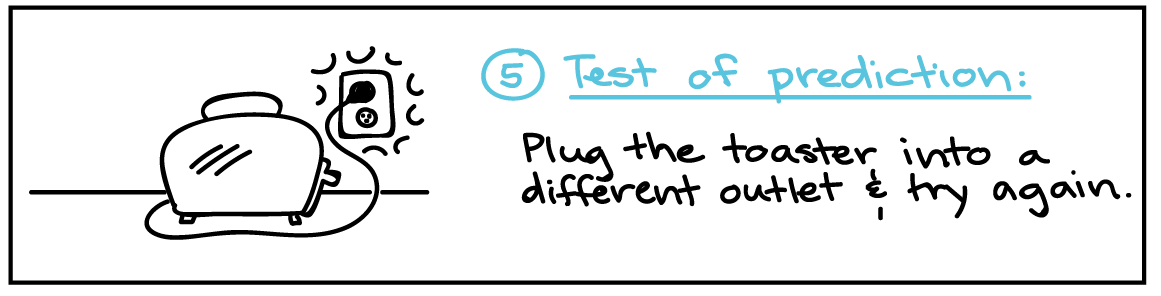
\includegraphics[scale=1]{toast_exp}
\end{frame}

\begin{frame}{Check the Results}
  \centering
  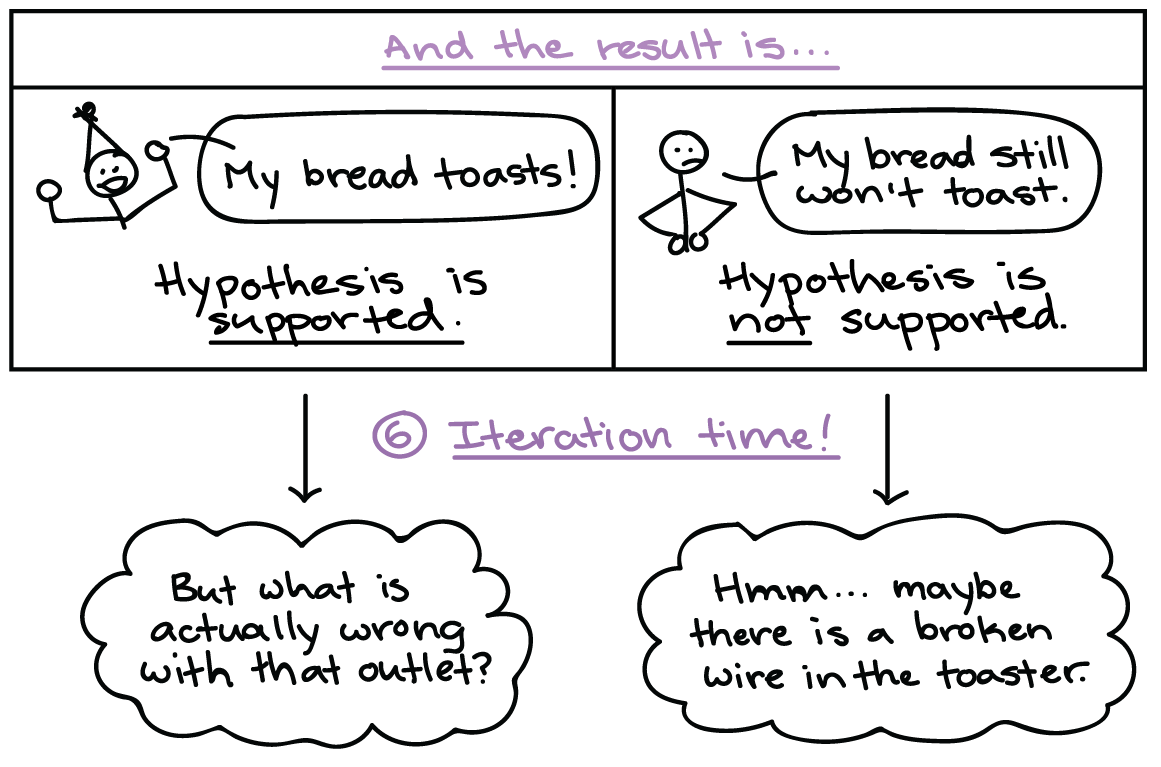
\includegraphics[scale=1]{toast_iterate}
\end{frame}

\section{Chapter 2}

\subsection{Dalton's Atomic Thoery}

\begin{frame}{Recall: Conservation of Mass}
  Any system closed to all transfers of matter and energy, the mass
  of the system must remain constant over time
\end{frame}

\begin{frame}{Dalton's Atomic Theory}
  \begin{enumerate}
  \item Elements consist of indivisible small particles (atoms)
  \item All atoms of the same element are identical and
    different elements have different types of atom
  \item Atoms can neither be created nor destroyed
  \item Compounds are formed when atoms of different
    elements join in simple ratios
  \end{enumerate}
\end{frame}

\subsection{Structure of the Atom}

\begin{frame}{Existence of the Electron}
  \begin{itemize}
  \item J.J. Thompson Cathode-ray experiment led to
    discovering of the electron
  \end{itemize}

  \centering
  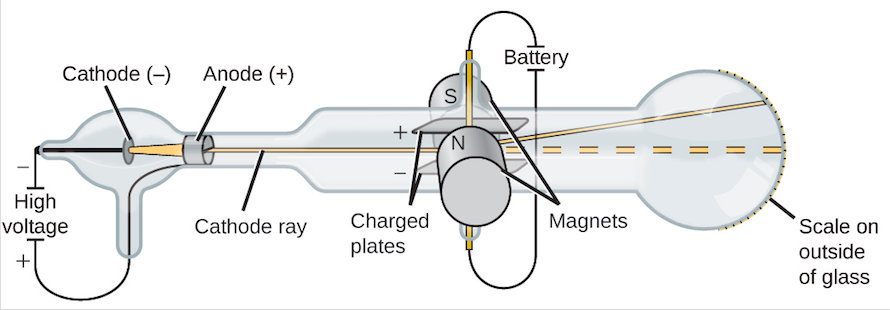
\includegraphics[scale=0.3]{cathod_ray}
\end{frame}

\begin{frame}{Millikan's Oil-Drop Experiment}
  \begin{center}
    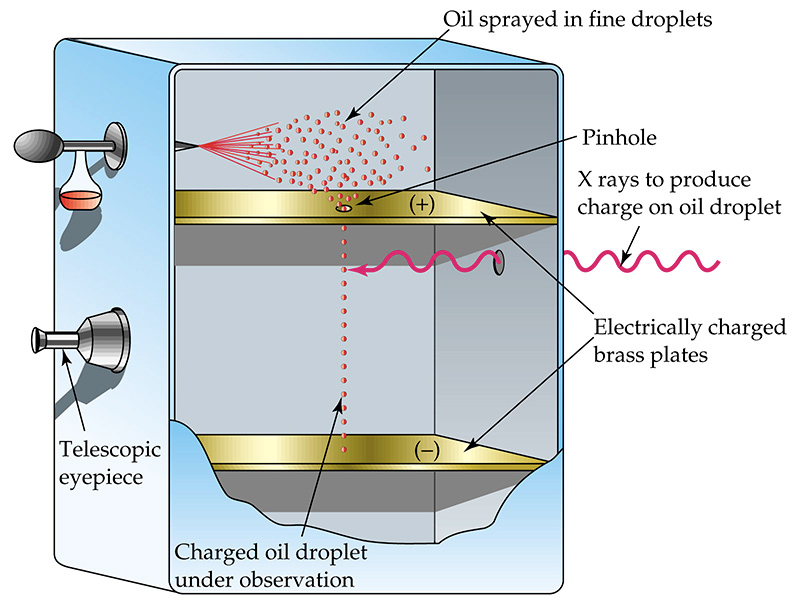
\includegraphics[scale=0.27]{millikin_oil}
  \end{center}

  \begin{itemize}
  \item Experiment determined the charge of an electron
    to be $-1.6022\times 10^{-19}$ Coulomb (C) and the mass to be
    $9.1094\times 10^{-28}$ g
  \end{itemize}
\end{frame}

\begin{frame}{J.J. Thompson's Plum Pudding Model}
  \centering
  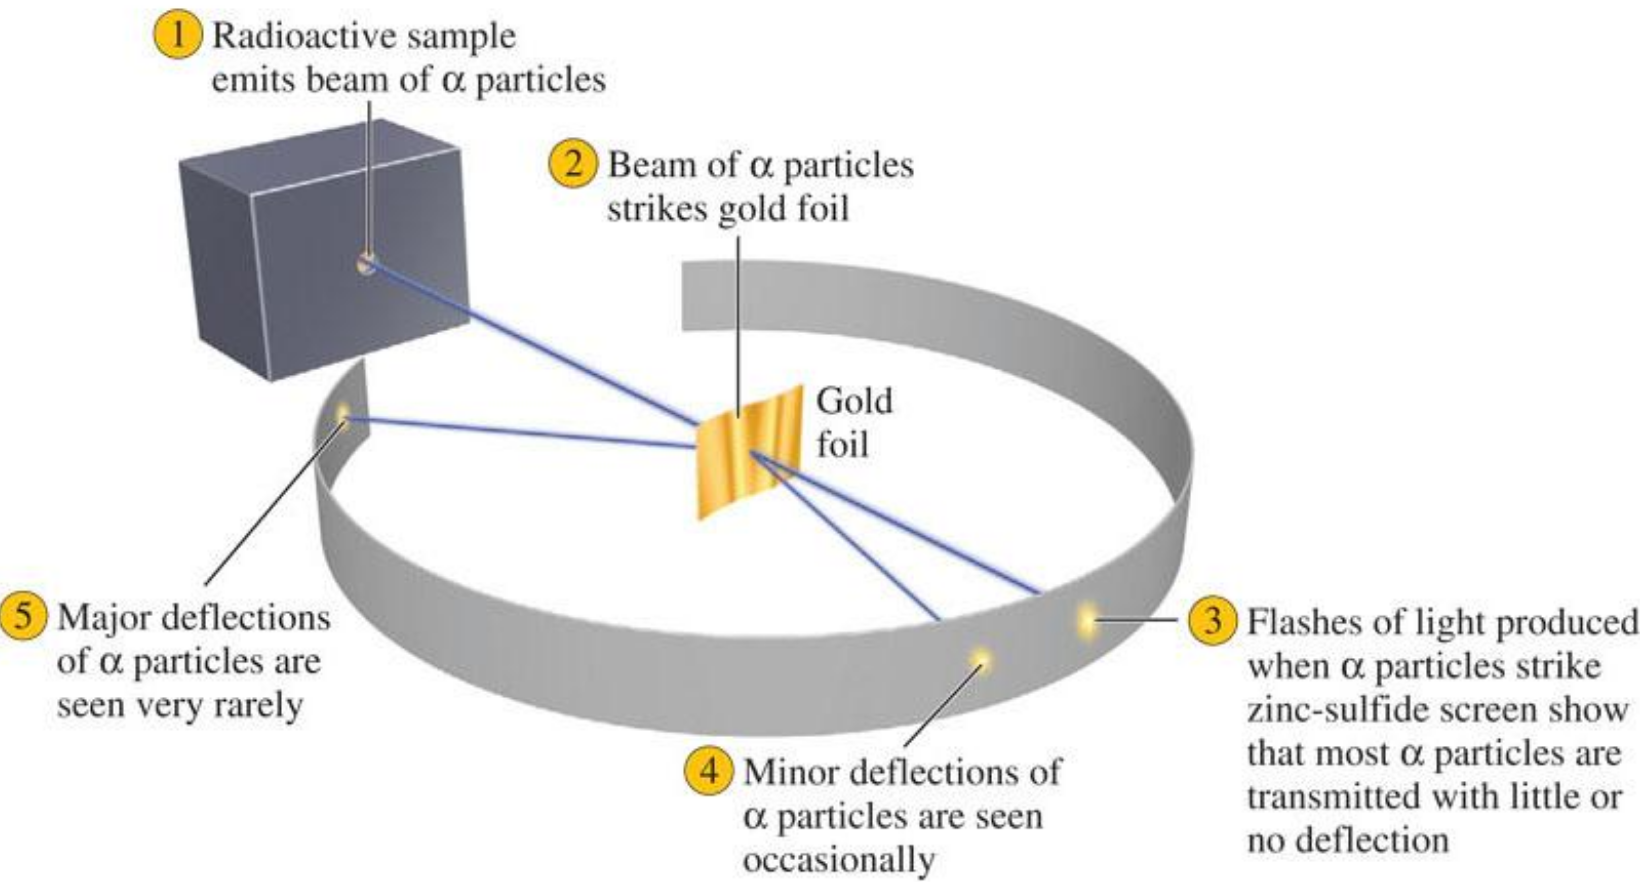
\includegraphics[scale=0.175]{alpha}
\end{frame}

\begin{frame}{J.J. Thompson's Plum Pudding Model}
  \centering
  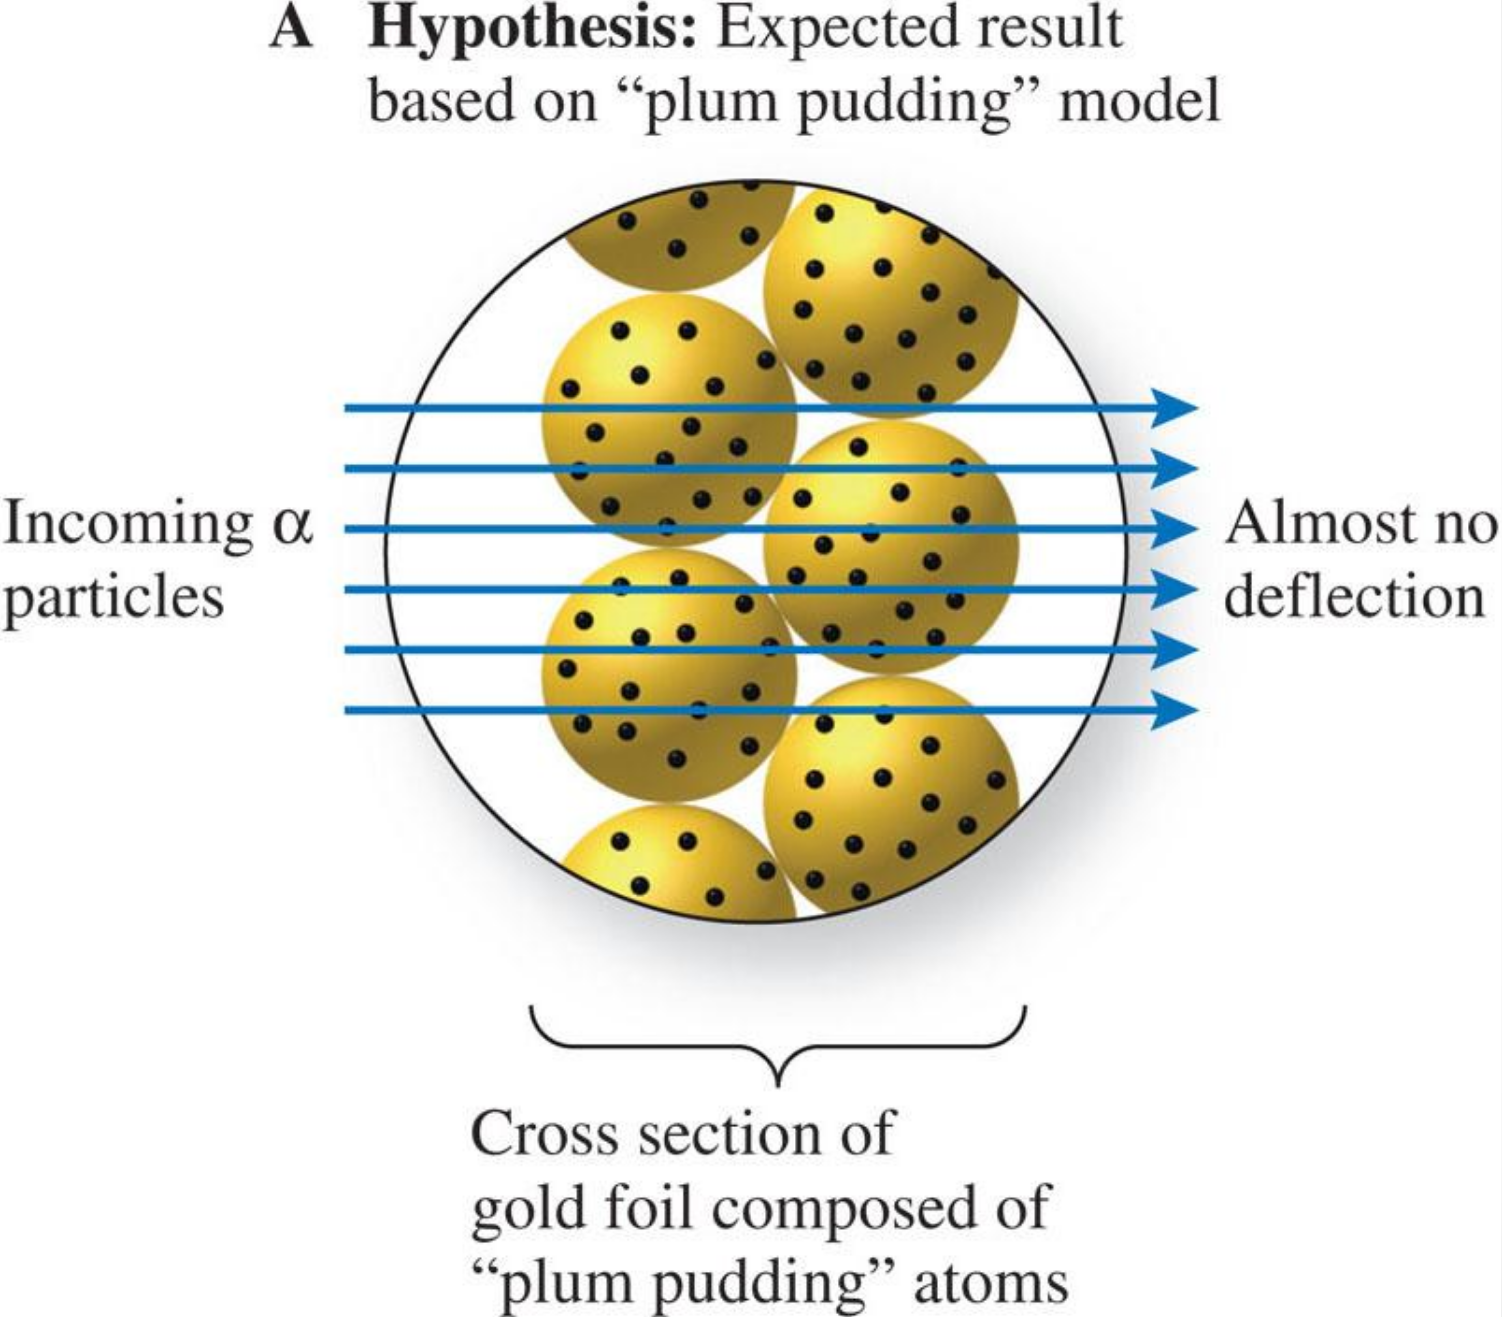
\includegraphics[scale=0.15]{test_hypothesis}
\end{frame}

\begin{frame}{J.J. Thompson's Plum Pudding Model}
  \centering
  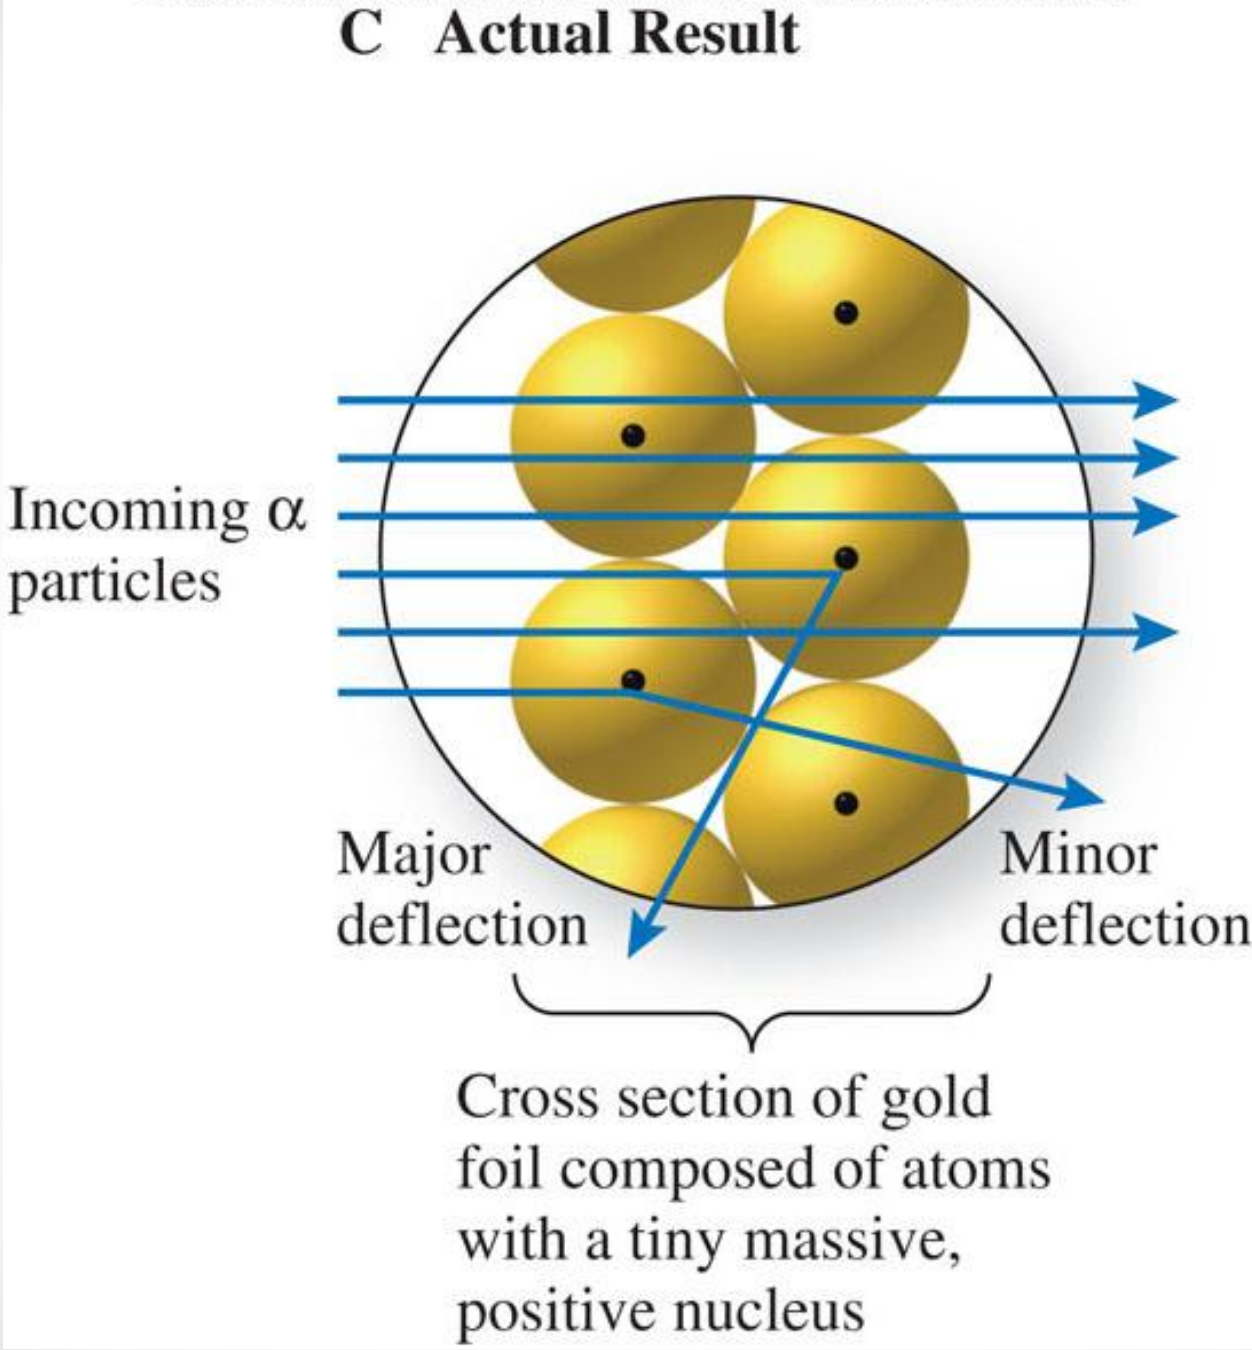
\includegraphics[scale=0.15]{reality}
\end{frame}

\begin{frame}{Existance of the Nucleus}
  \begin{itemize}
  \item Plum pudding model is not valid
  \item Nuclear model is developed where the diameter of the nucleus
    is $\sim 10^{-14}$ m and the diameter of the atom is $\sim 10^{-10}$ m
  \item \textbf{Question:} If an atom is made of mostly space,
    why can't we walk through anything?
  \end{itemize}
\end{frame}

\begin{frame}{What are atoms made of?}
  \centering
  \begin{tabular}{c|ccc}
    & Mass (g) & Atomic Units (Amu) & Charge (C) \\
    \hline
    Neutron  & $1.675\times 10^{-24}$ & 1 & 0 \\
    Proton   & $1.675\times 10^{-24}$ & 1 & $1.6022\times 10^{-19}$ \\
    Electron & $9.1094\times 10^{-28}$ & 1/1840 & $-1.6022\times 10^{-19}$
  \end{tabular}

  \begin{itemize}
  \item 1 amu = $1.6606 \times 10^{-24}$ g
  \item Protons and neutrons are located in the nucleus
  \item Electrons revolve around the nucleus (difference between
    core electrons and valence electrons)
  \end{itemize}
\end{frame}

\subsection{Ions and Atomic Mass}

\begin{frame}{What are ions?}
  \begin{center}
    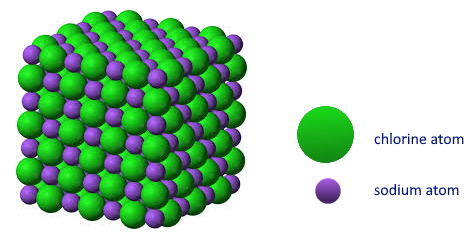
\includegraphics[scale=0.5]{nacl}
  \end{center}

  \begin{itemize}
  \item When an atom loses (cation) or gains (anion) an electron
  \end{itemize}
\end{frame}

\begin{frame}{Defining Atomic Number and Mass}
  \begin{equation}
    ^\text{A}_\text{Z}\text{X}^\text{C}
  \end{equation}

  where A is the atomic mass, Z is the atomic number, X is atomic
  symbol, and C is the overall charge
\end{frame}

\begin{frame}{Reminder: Periodic Table}
  \centering
  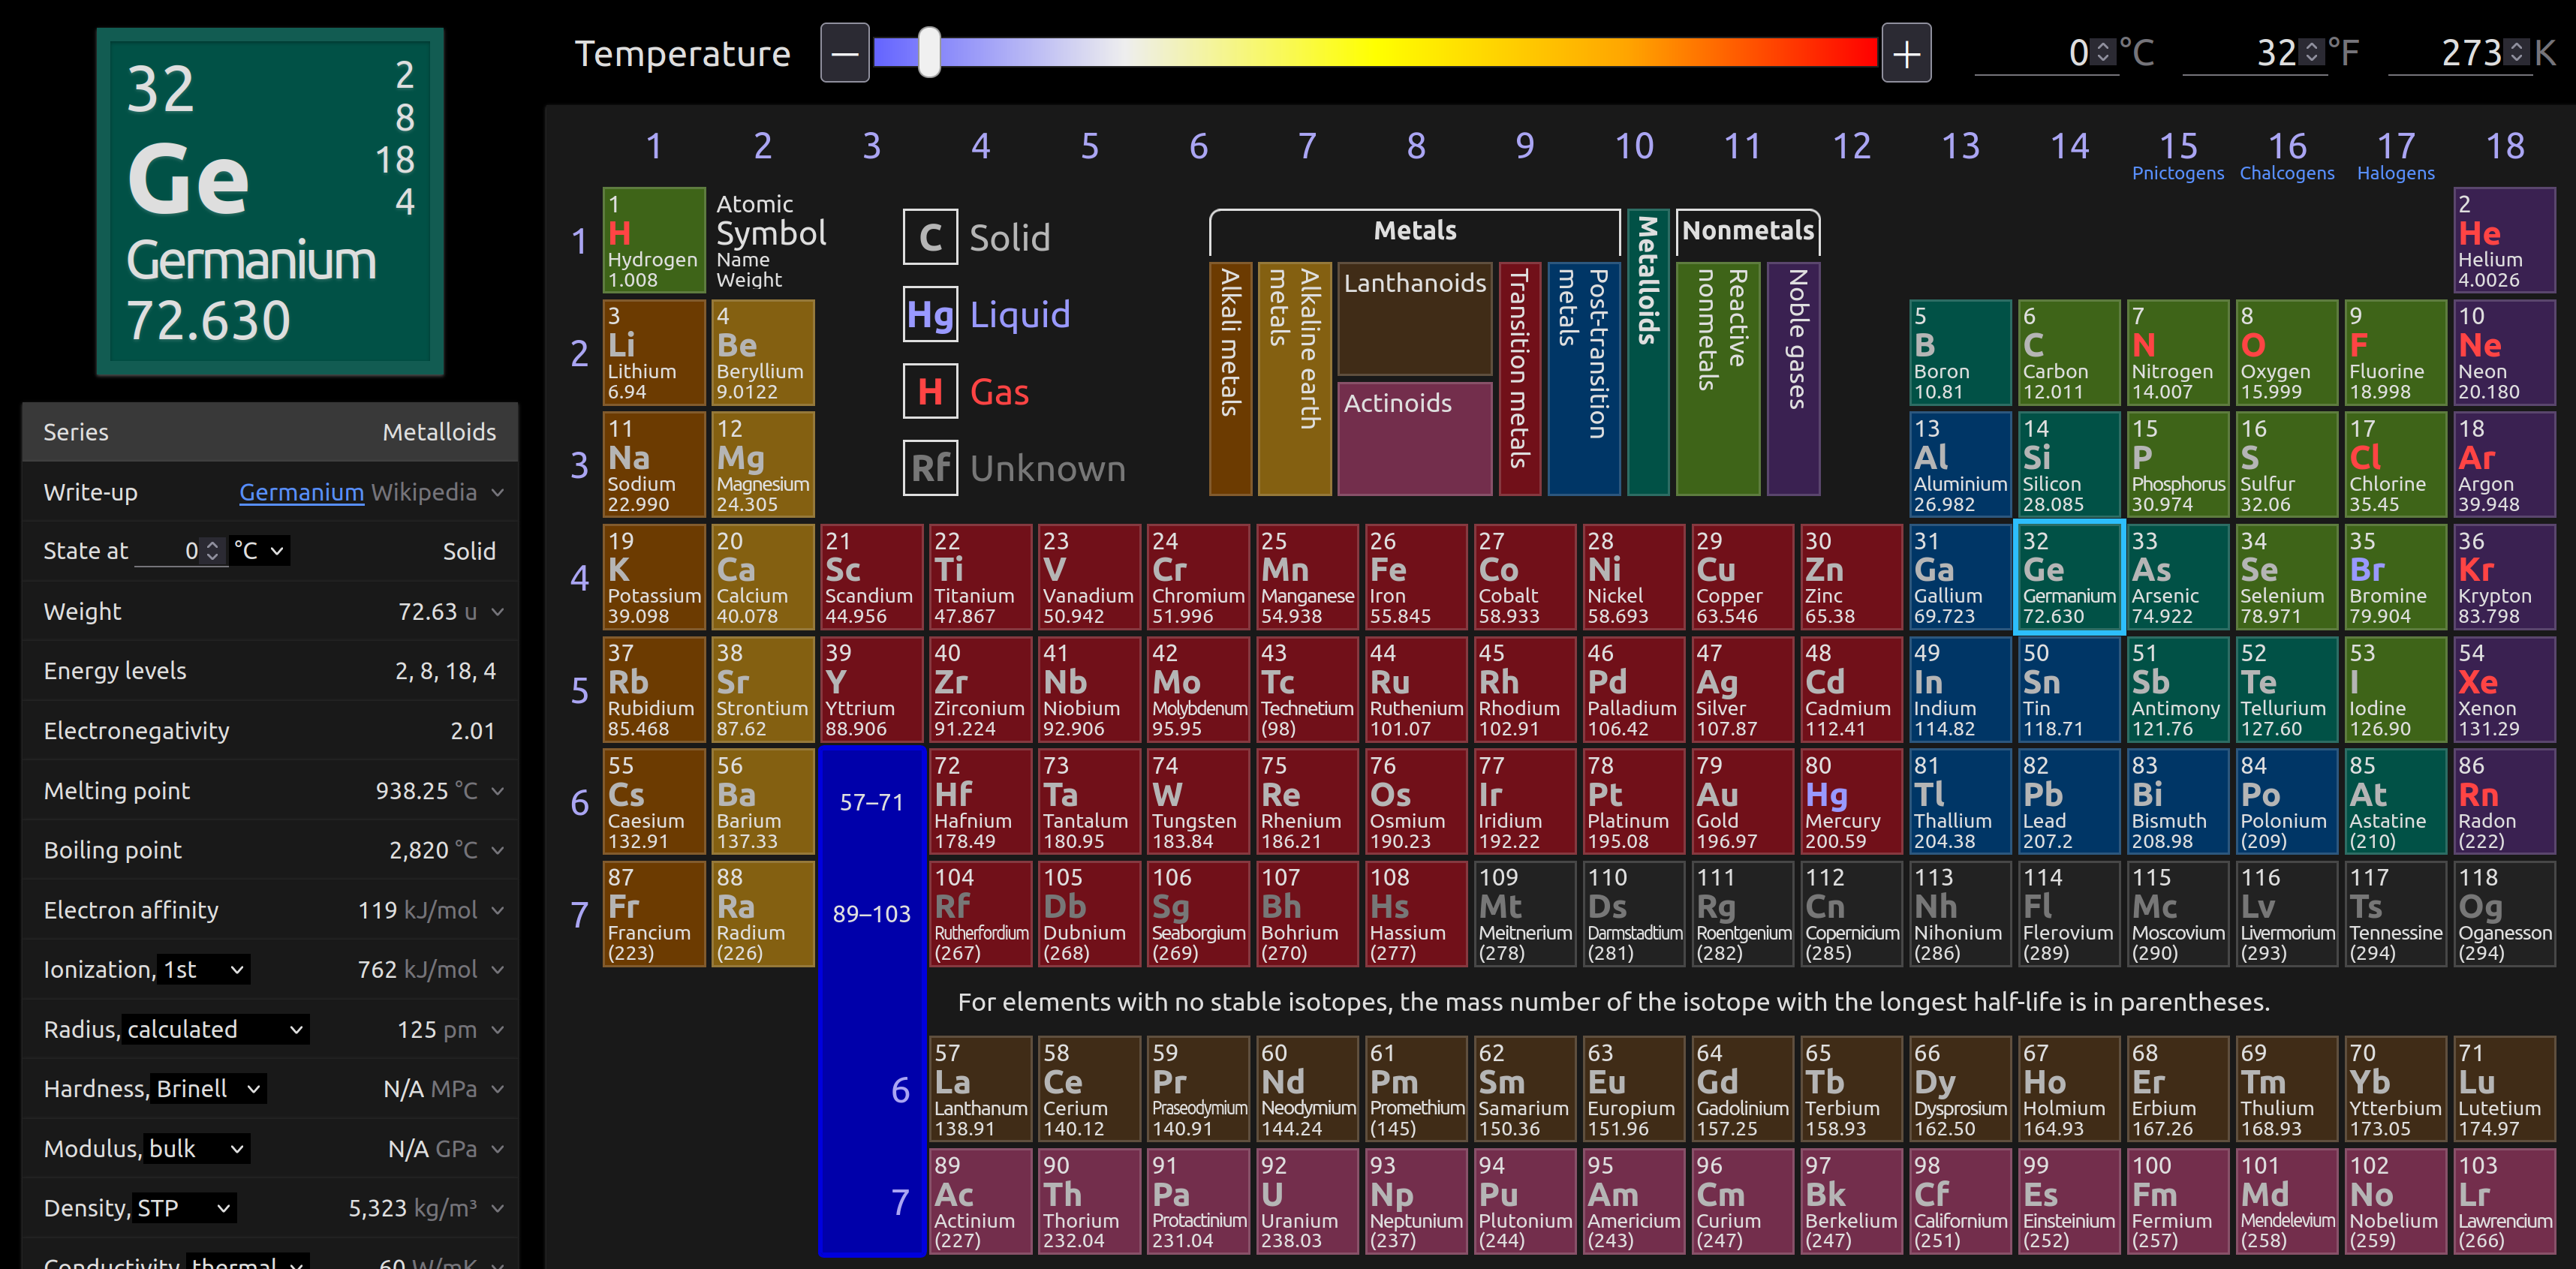
\includegraphics[scale=0.3]{ptable}
\end{frame}

\begin{frame}{Practice: Write the Nuclear Symbol}
  \begin{itemize}
  \item Ge - atomic mass: 72
  \item He - atomic mass: 2
  \item Ge$^{3+}$ - atomic mass: 72
  \item Br$^{-}$ - atomic mass: 79
  \item S$^{2-}$ - atomic mass: 32
  \end{itemize}
\end{frame}

\begin{frame}{Isostopes: Revisiting the Neutron}
  \begin{center}
    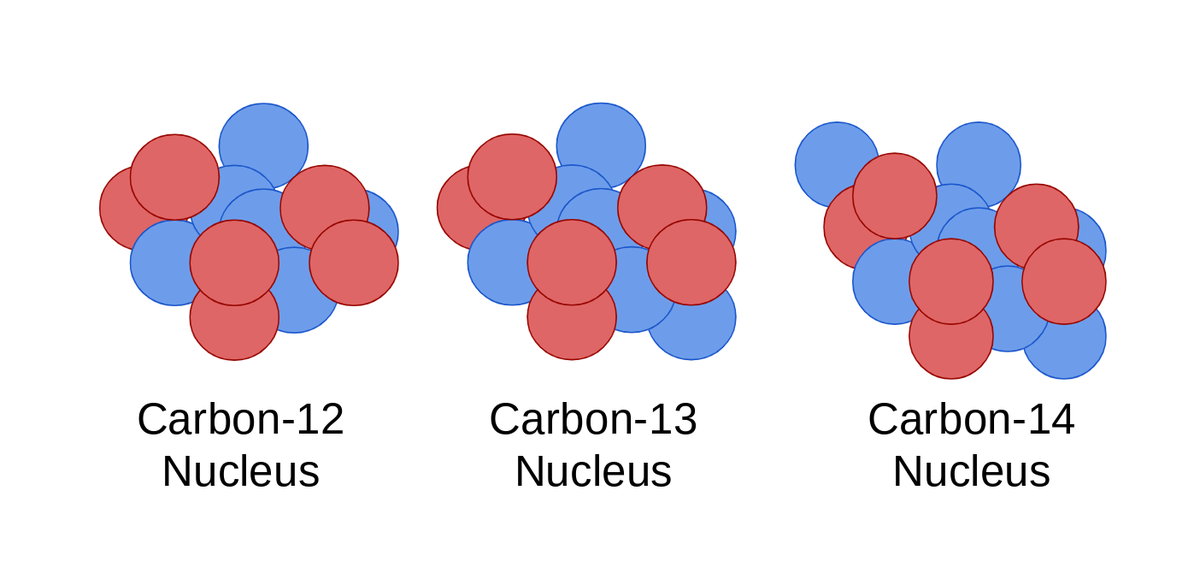
\includegraphics[scale=0.2]{carbon_isotopes}
  \end{center}
  where red is the proton and blue is the neutron
  
  \begin{itemize}
  \item Same number of protons (Z)
  \item Different number of neutrons leading to
    a different atomic mass (A)
  \item \textbf{Practice:} Write the Nuclear Symbol for
    C-12, C-13, and C-14
  \end{itemize}
\end{frame}

\subsection{Periodic Table}

\begin{frame}{Earliest Periodic Table}
  \begin{center}
    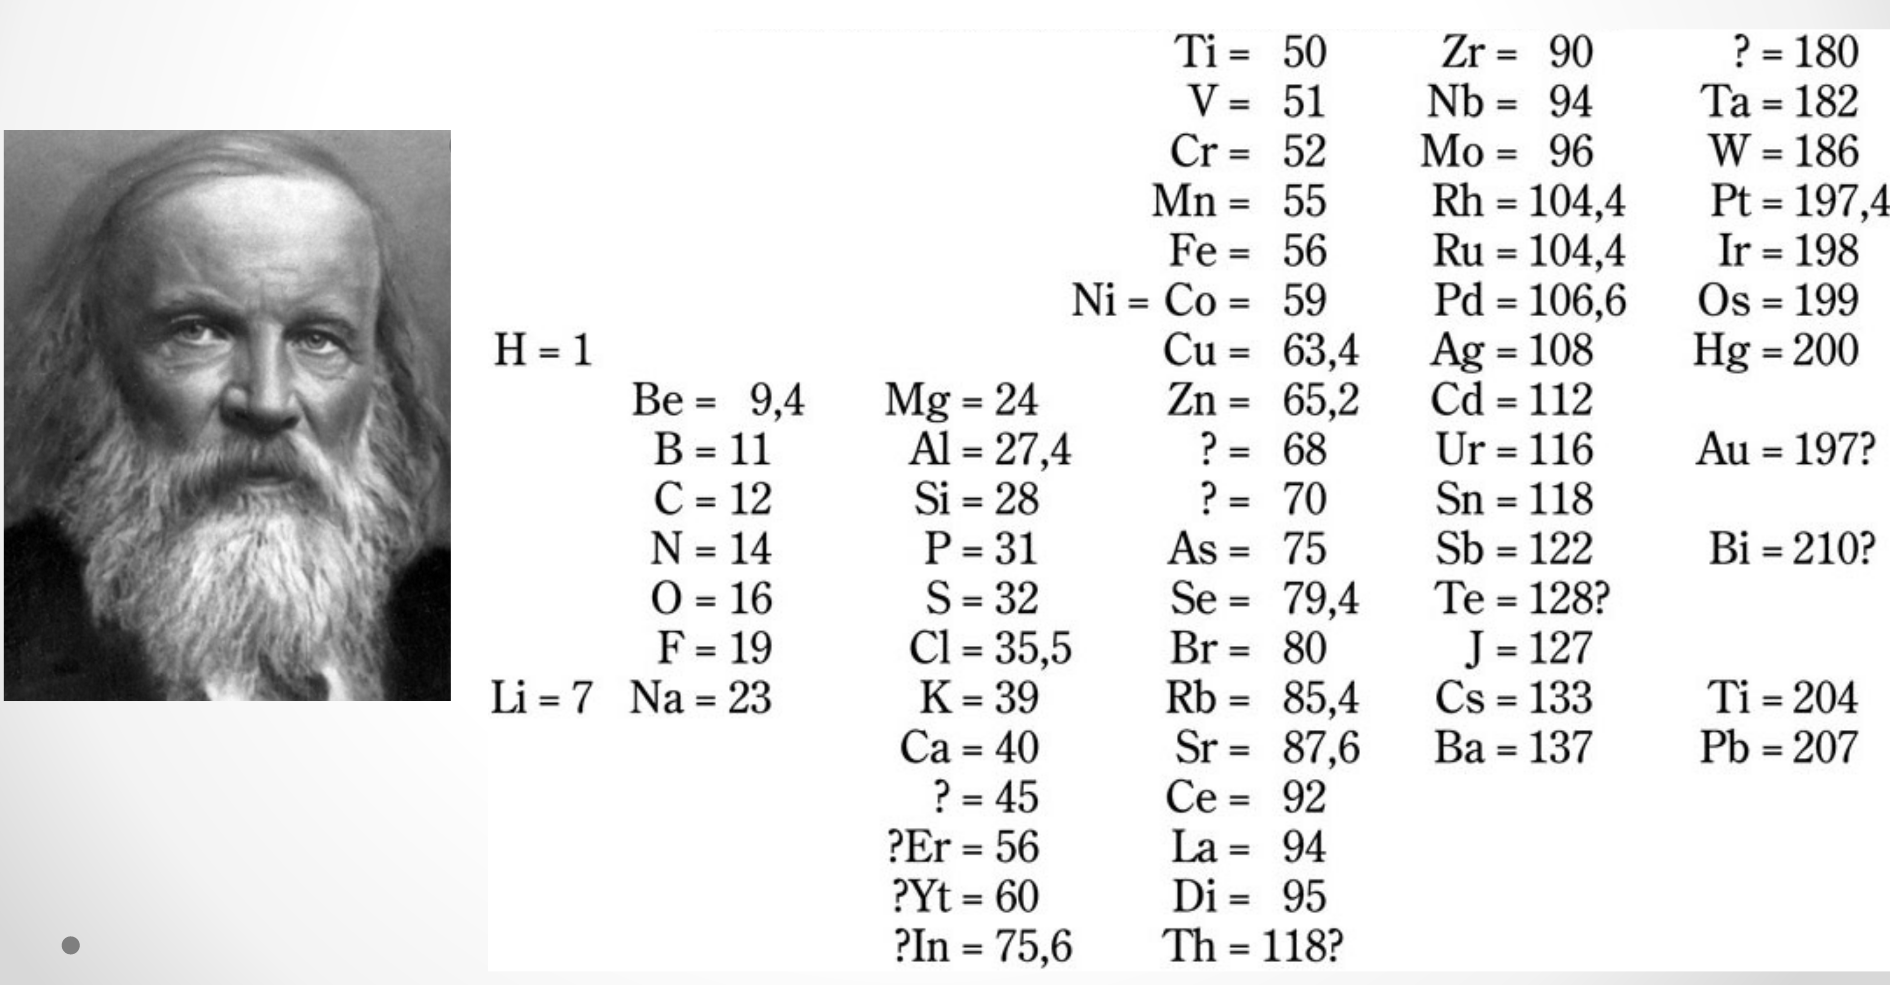
\includegraphics[scale=0.13]{mendeleev_table}
  \end{center}
  
  \begin{itemize}
  \item Dmitrij Mendeleev Arranged base on atomic mass
  \item Grouped known elements into rows and columns
  \end{itemize}
\end{frame}

\begin{frame}{Modern Period Table}
  \centering
  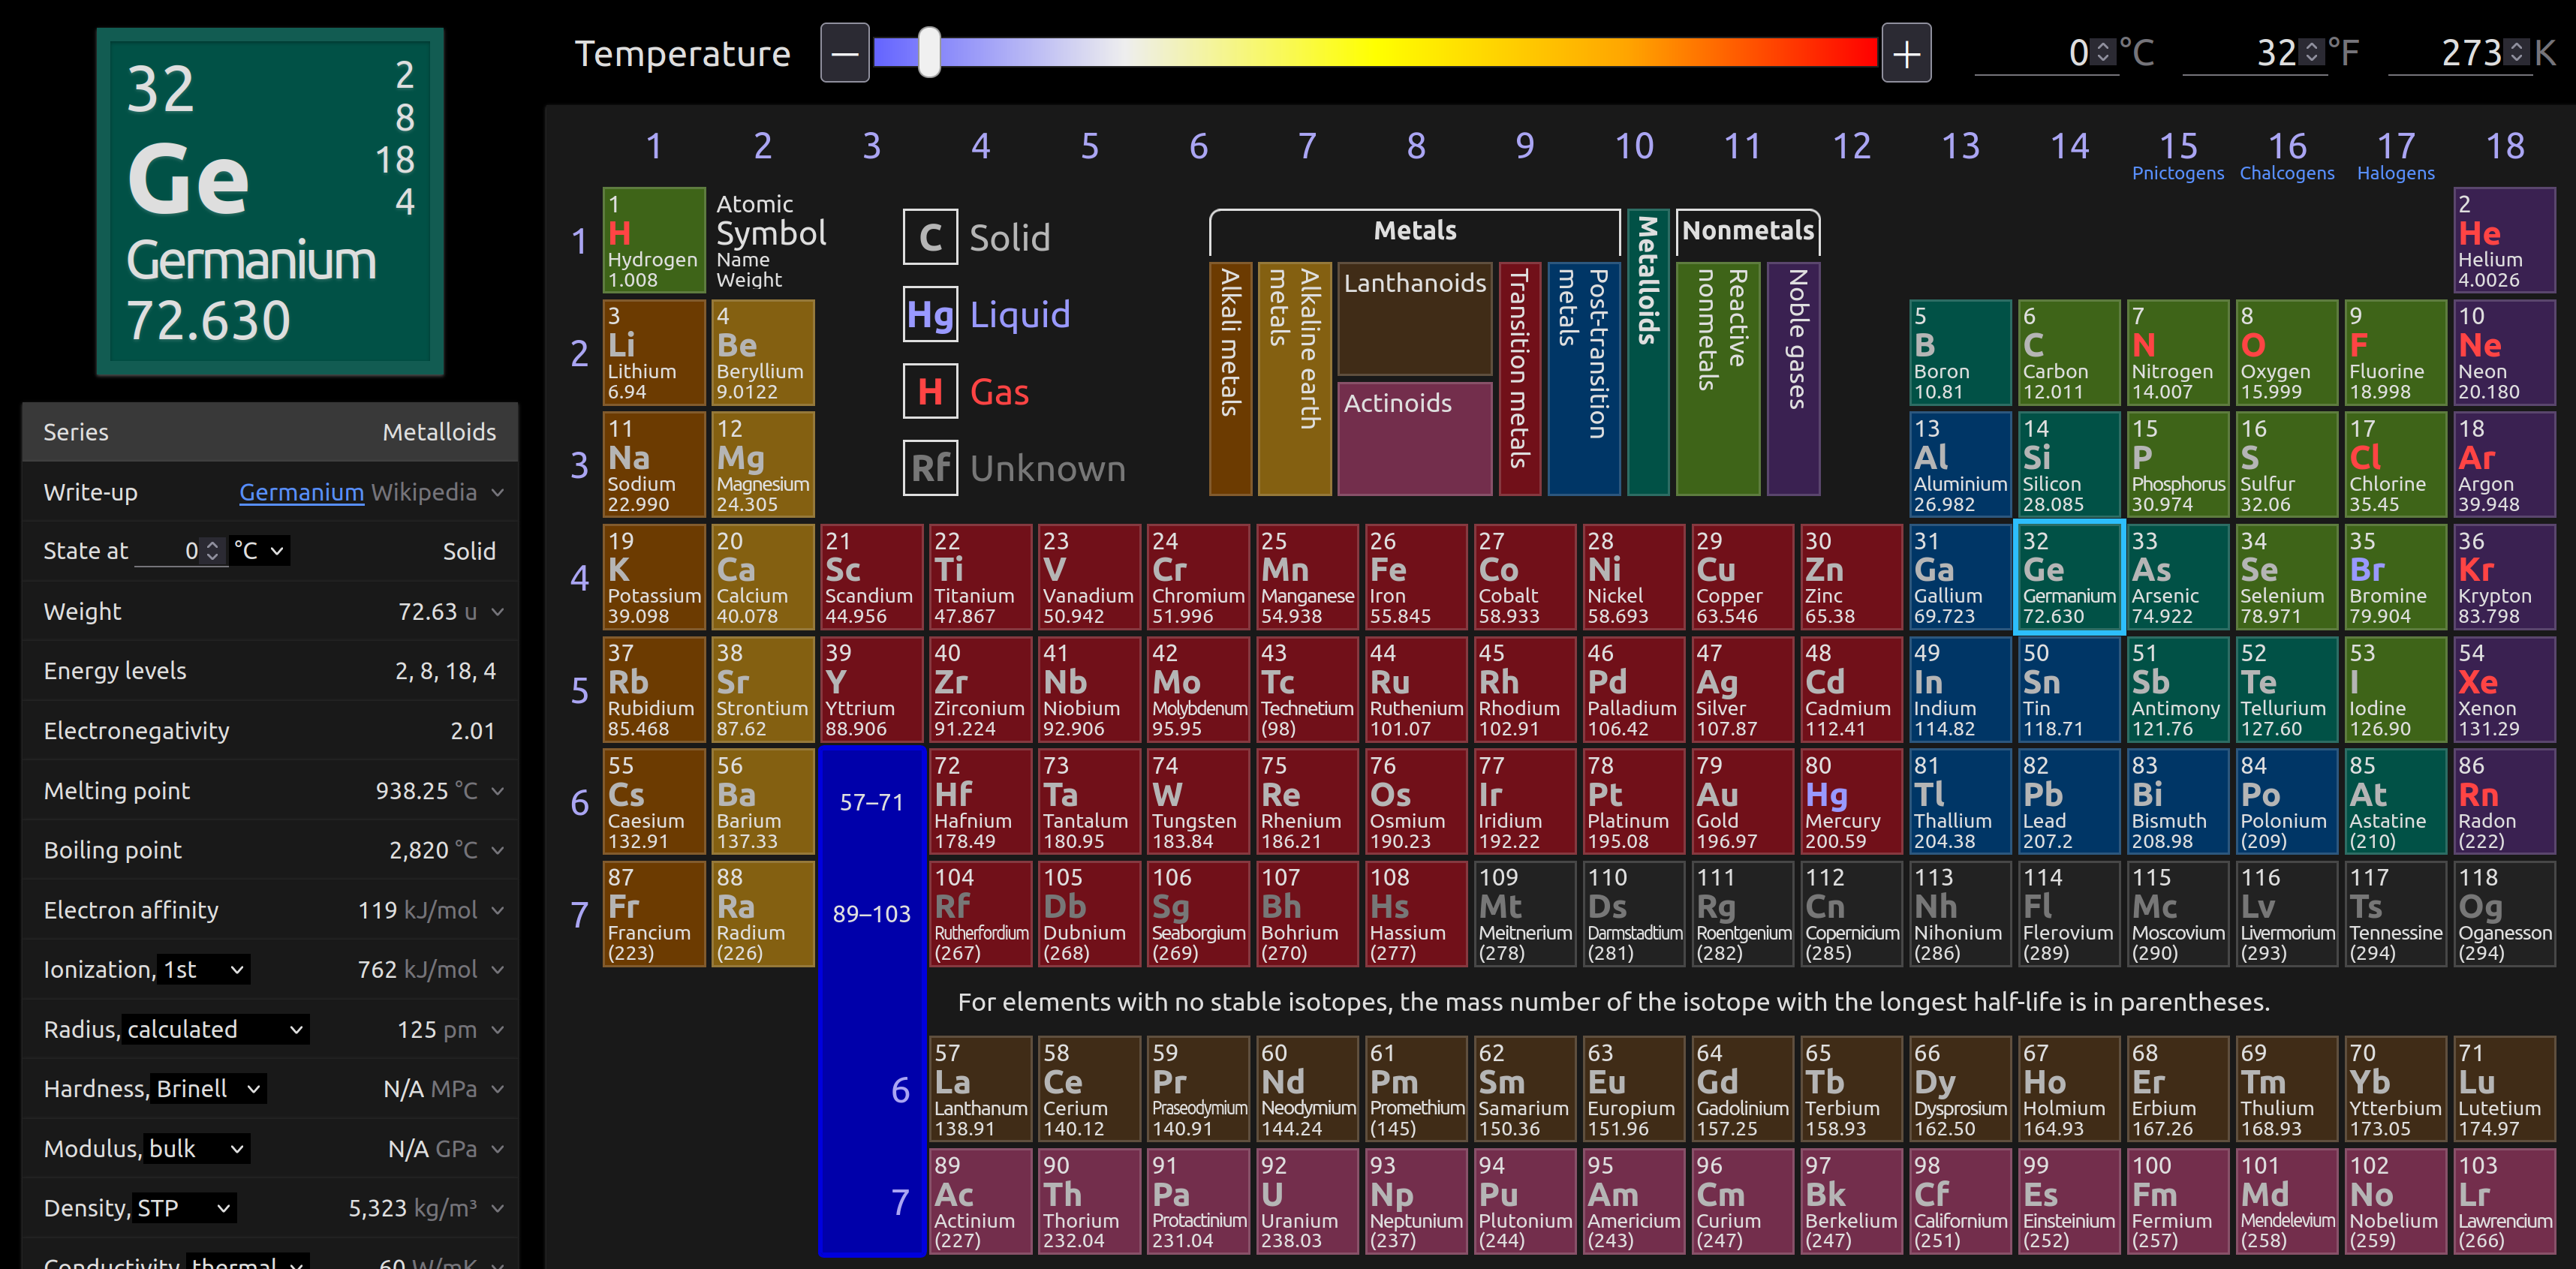
\includegraphics[width=\linewidth]{ptable}
\end{frame}

\begin{frame}{Mass Spectroscopy: Determining the Atomic Mass}
  \begin{center}
    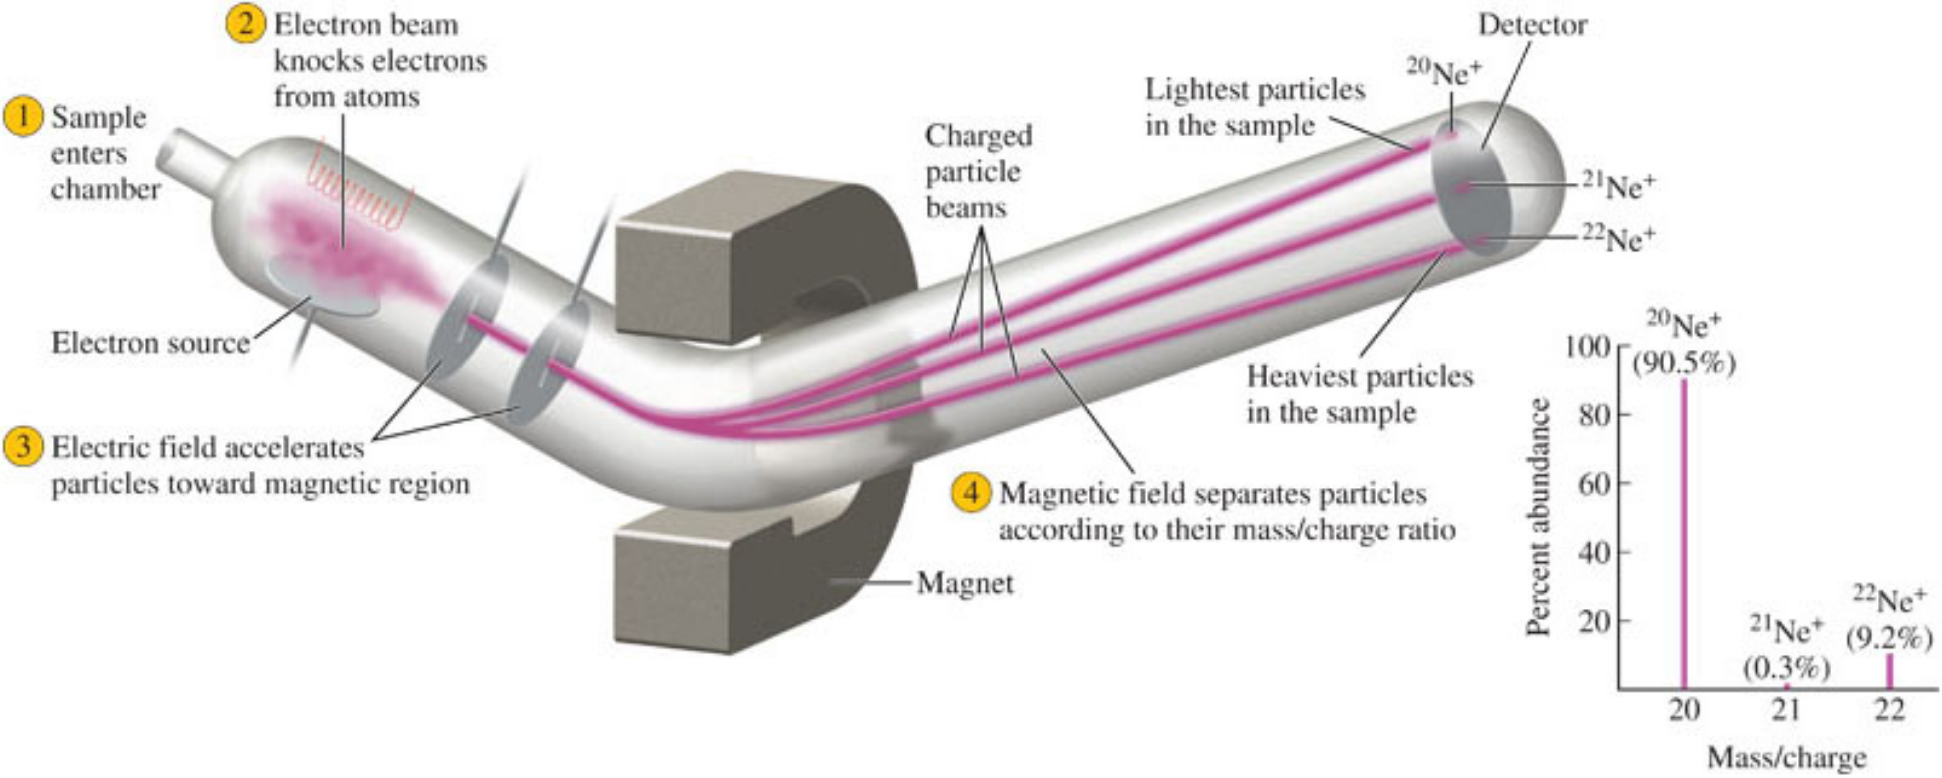
\includegraphics[width=\linewidth]{mass_spect}
  \end{center}

  \begin{itemize}
  \item Ionizes the atom and electric field accelerates atoms
  \item Time of flight - heavier atoms will travel slower
    than lighter ones
  \item Weighter average of atomic masses
  \end{itemize}
\end{frame}

\begin{frame}{Relative Atomic Mass Formula}
  \begin{equation}
    \text{Relative Atomic Mass} = (I_1\times A_1) + (I_2\times A_2) + \dots
  \end{equation}
  where $I$ is the mass of the isotope, and $A$ is the
  relative abundance between 0 and 1
\end{frame}

\begin{frame}{Calculating the Relative Atomic Masses}
  Magnesium is composed of three isotopes. Calculate the
  relative atomic mass of magnesium and compare to the periodic
  table.
  \begin{center}
  \begin{tabular}{ccc}
    Isotope & Mass (amu) & Natural Abundance ($\%$) \\
    \hline
    $^{24}$Mg & 23.985 & 78.99 \\
    $^{25}$Mg & 24.986 & 10.00 \\
    $^{26}$Mg & 25.983 & 11.01
  \end{tabular}
  \end{center}
\end{frame}

\begin{frame}{Calculating the Relative Atomic Masses}
  Magnesium is composed of three isotopes. Calculate the
  relative atomic mass of magnesium and compare to the periodic
  table.
  \begin{center}
  \begin{tabular}{ccc}
    Isotope & Mass (amu) & Natural Abundance ($\%$) \\
    \hline
    $^{24}$Mg & 23.985 & 78.99 \\
    $^{25}$Mg & 24.986 & 10.00 \\
    $^{26}$Mg & 25.983 & 11.01
  \end{tabular}
  \end{center}

  \begin{align*}
    23.985\text{amu}\times 0.7899 & =  18.95 \text{amu} \\
    24,986\text{amu}\times 0.1000 & =  2.499 \text{amu} \\
    25.983\text{amu}\times 0.1101 & =  2.861 \text{amu} \\
    \hline
    &   24.31 \text{amu}
  \end{align*}
\end{frame}

\begin{frame}{Practice: Calculate the Atomic Mass}
  Boron has two naturally occuring isotopes. Determine the
  atomic mass of boron.
  
  \begin{center}
  \begin{tabular}{cc}
    Isotope & Natural Abundance ($\%$) \\
    \hline
    $^{10}$B & 19.9 \\
    $^{11}$B & 80.1 
  \end{tabular}
  \end{center}
\end{frame}

\begin{frame}{Practice: Calculate the Atomic Mass}
  \begin{center}
    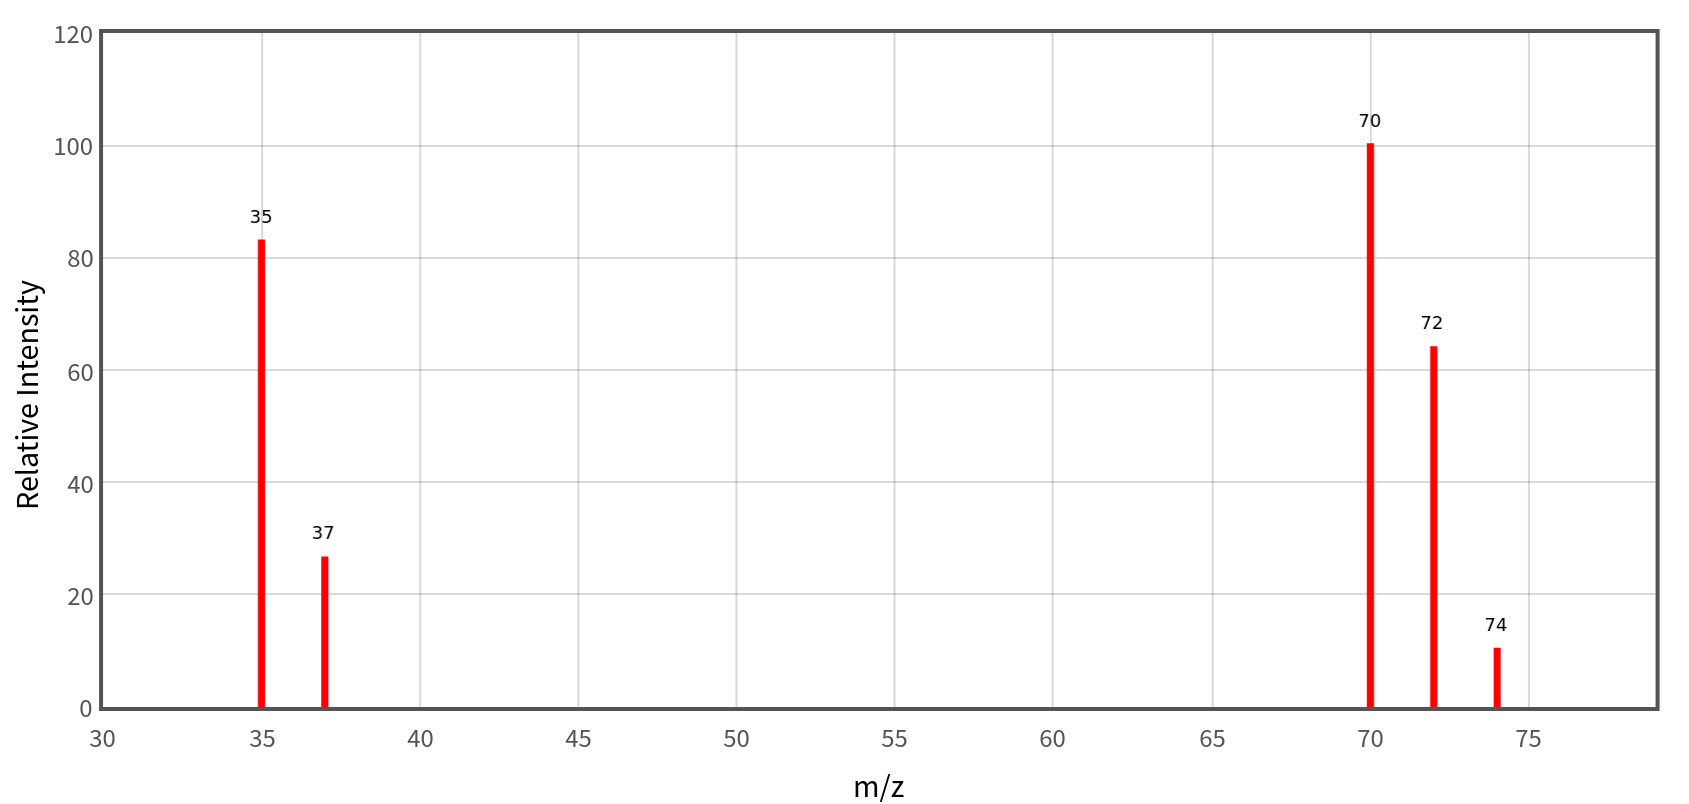
\includegraphics[scale=0.175]{cl_mass_spec}
  \end{center}
  Determine atomic mass of Cl given the mass spectrum. Hint:
  Cl naturally exists as a diatomic e.g. Cl$_2$.
\end{frame}

\begin{frame}{Conceptual Question}
  Naturally occurring gallium (ga) is made of two isotopes
  Ga-69 and Ga-71. Which of the following statements is true?
  Hint: Look at the periodic table.
  
  \begin{enumerate}
  \item Gallium's relative atomic mass is 70.00 amu
  \item Both isotopes have the same mass: 69.72 amu
  \item The isotopes are present in the same percentages
  \item Ga-71 is present in the largest percent abundance
  \item Ga-69 is present in the largest percent abundance
  \end{enumerate}
\end{frame}

\begin{frame}{Alkali Metal}
  \begin{center}
    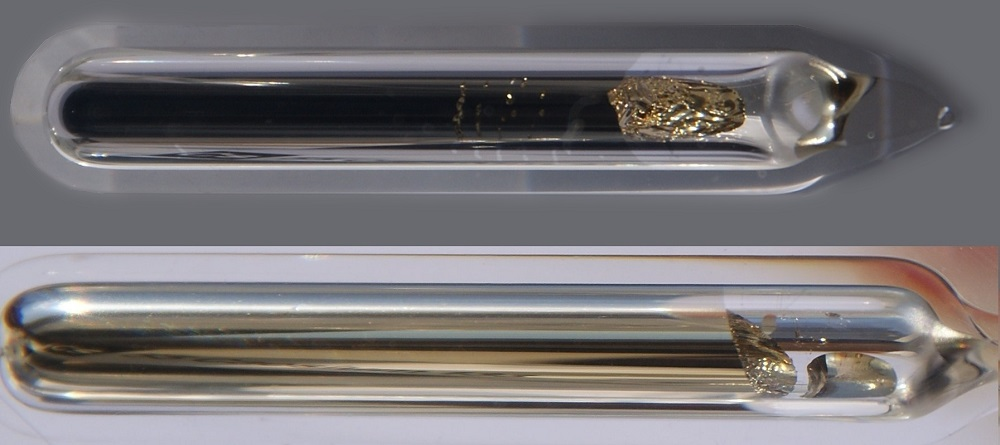
\includegraphics[scale=0.2]{alkali_metal}
  \end{center}
  
  \begin{itemize}
  \item Lower densities than other metals
  \item Extremely soft metals
  \item Highly reactive e.g. forming H$_2$ when in
    contact with water
  \item Prefer to lose an electron
  \end{itemize}
\end{frame}

\begin{frame}{Alkaline Earth Metal}
  \begin{center}
    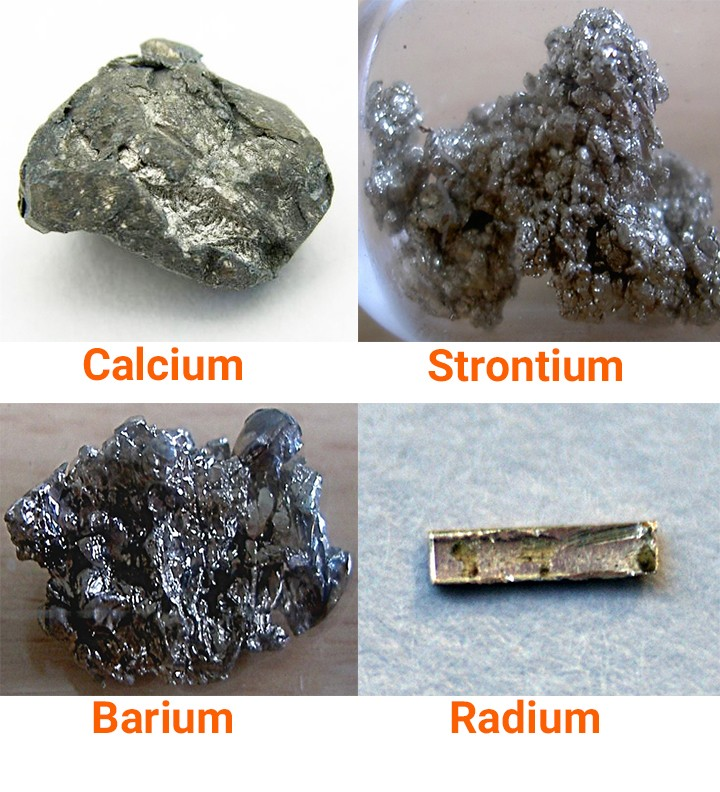
\includegraphics[width=0.4\linewidth]{alkaline_metal}
  \end{center}
  
  \begin{itemize}
  \item Fairly reactive metals
  \item Can form solutions with a pH greater than
    7 (more basic or alkaline)
  \item Calcium and magnesium important for life
  \item Prefer to lose 2 electrons
  \end{itemize}
\end{frame}

\begin{frame}{Transition Metals}
  \begin{center}
    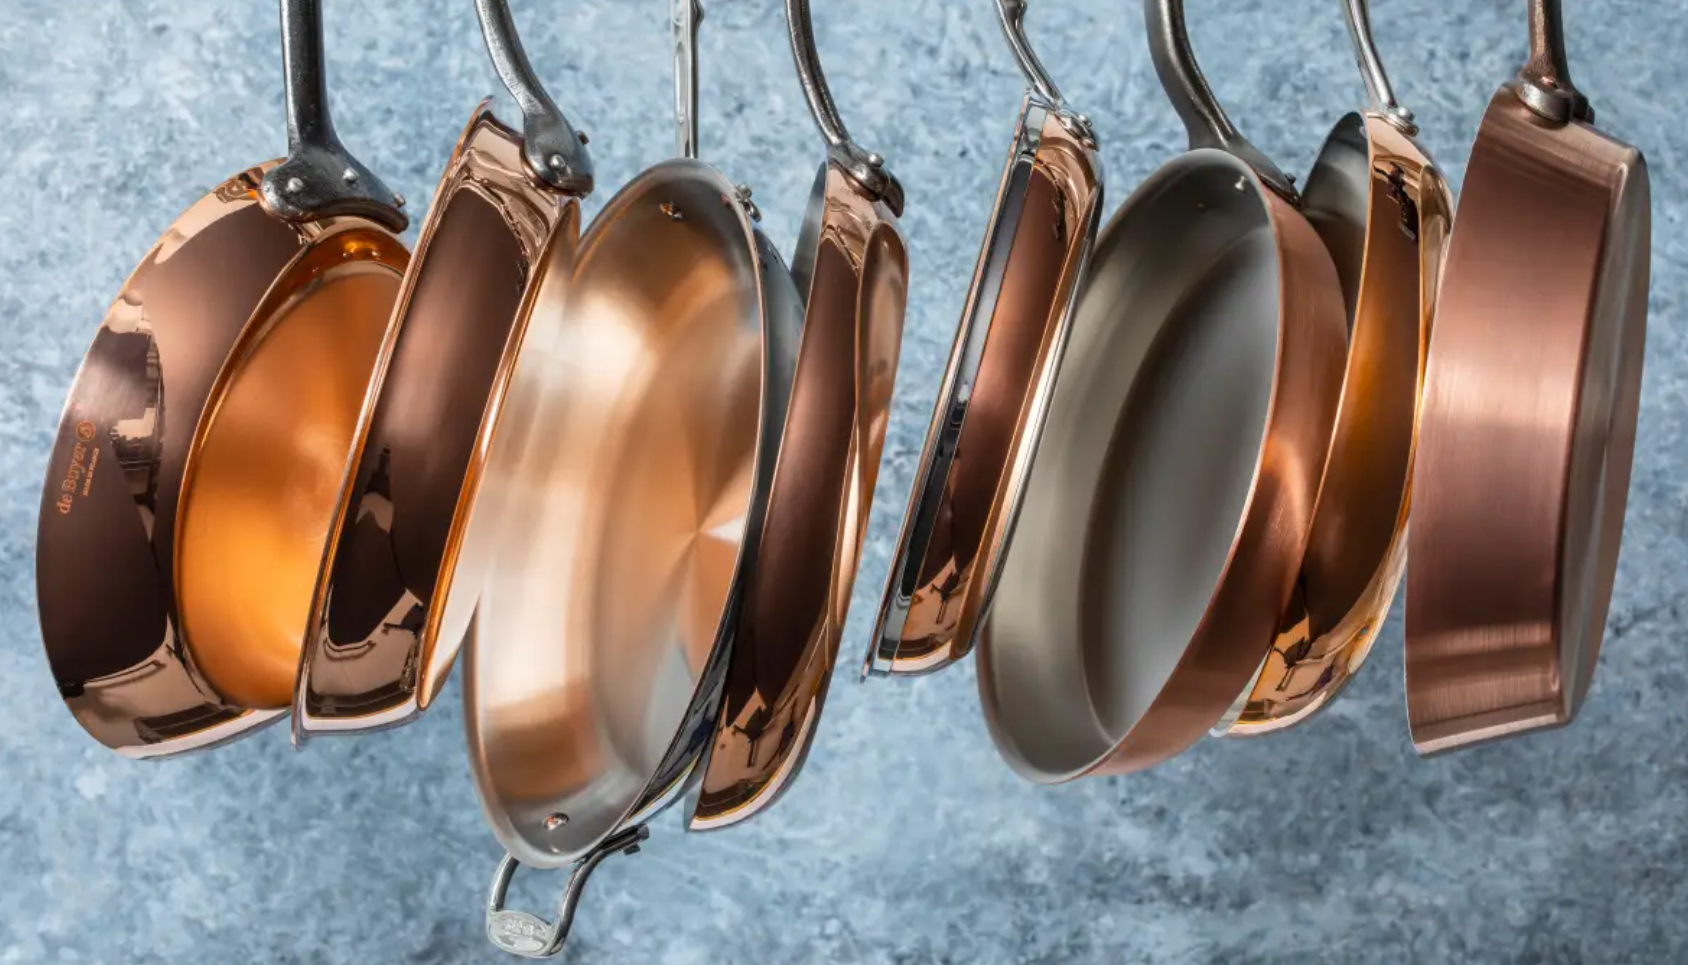
\includegraphics[scale=0.12]{copper_pan}
  \end{center}
  
  \begin{itemize}
  \item Easily malleable and great conductors of heat and
    electricity
  \item High melting points except mercury (liquid at Room
    temperature)
  \item High densities
  \item Oxidation states (ability to lose electrons) can
    vary between 1+ to 6+
  \end{itemize}
\end{frame}

\begin{frame}{Actinides and Lanthanides}
  \begin{center}
    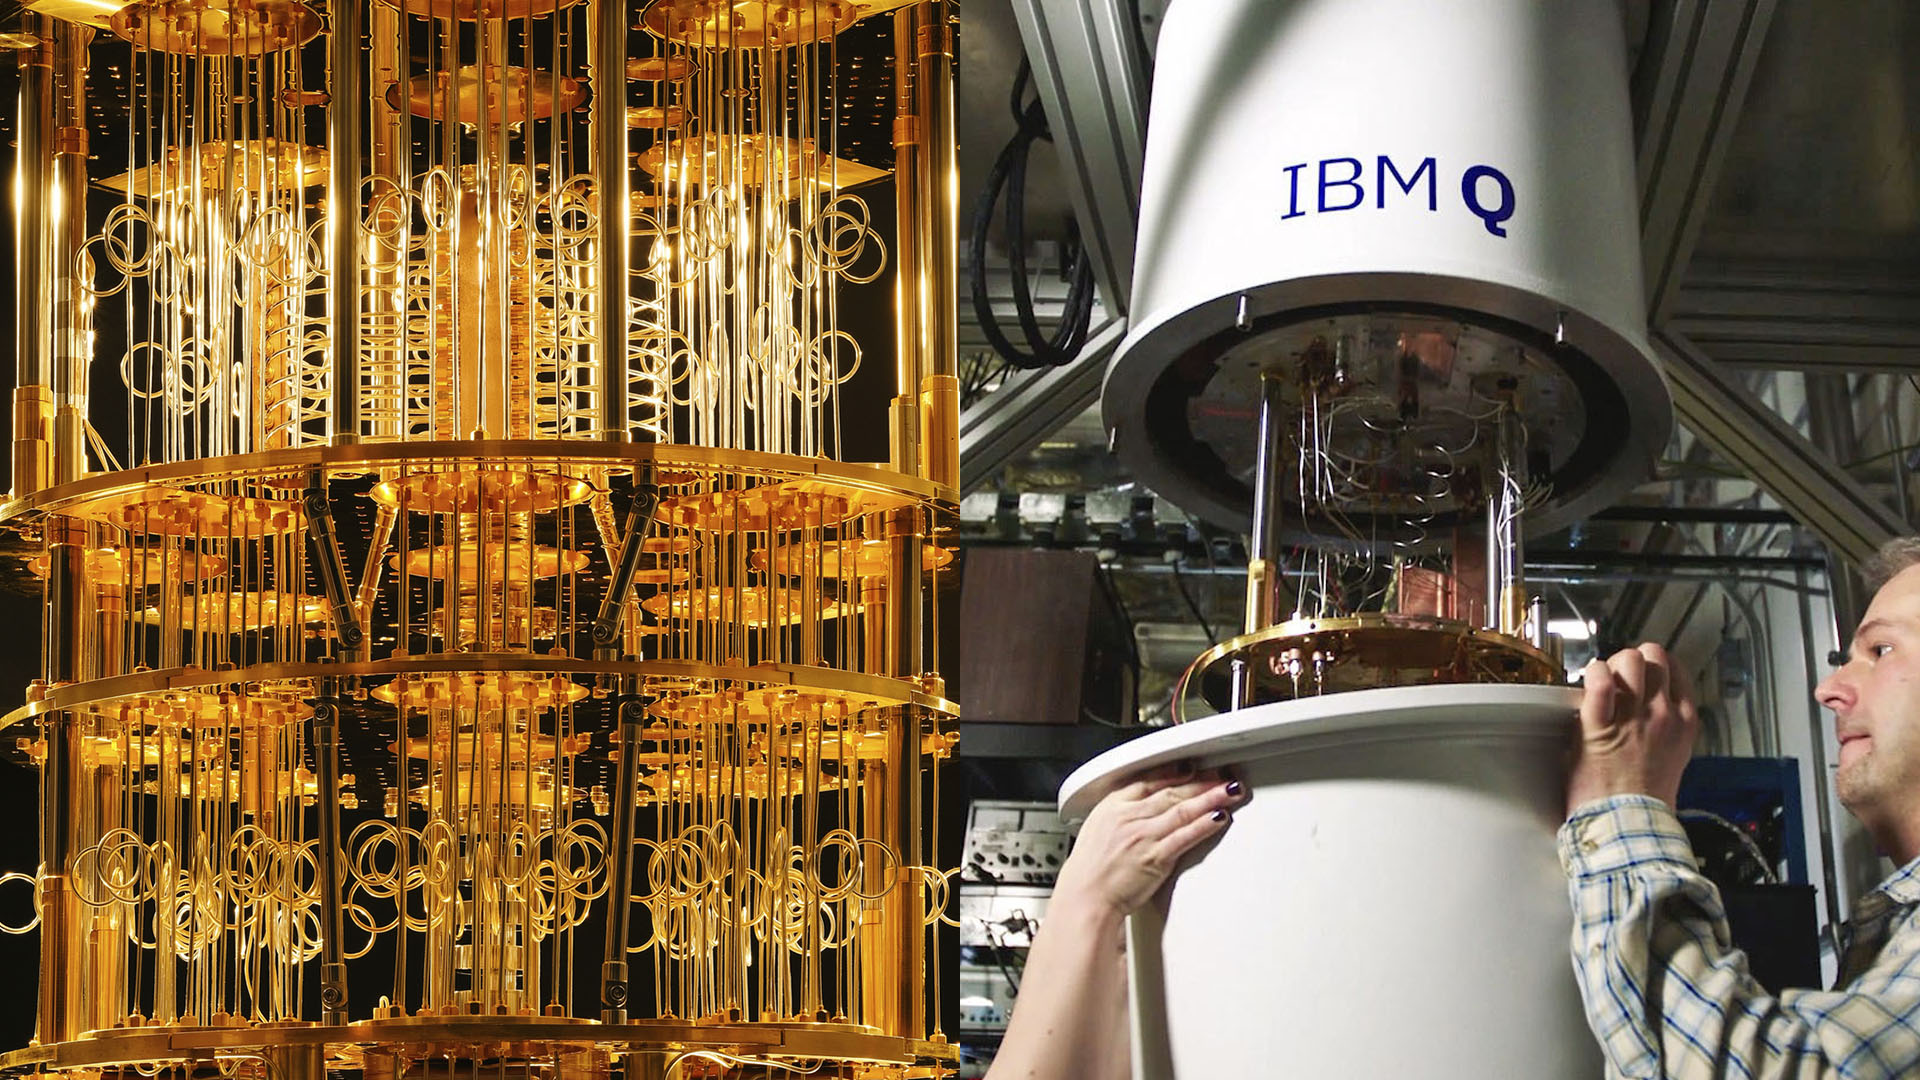
\includegraphics[scale=0.3]{quantum_comp}
  \end{center}

  \begin{itemize}
  \item Radioactive due to instability
  \item Silvery/silvery-white luster in metallic form
  \item Potential application to quantum computers and
    nuclear power
  \item Oxidation states can range from 2+ to 7+
  \end{itemize}
\end{frame}

\begin{frame}{Nuclear Power Plants}
  \begin{center}
    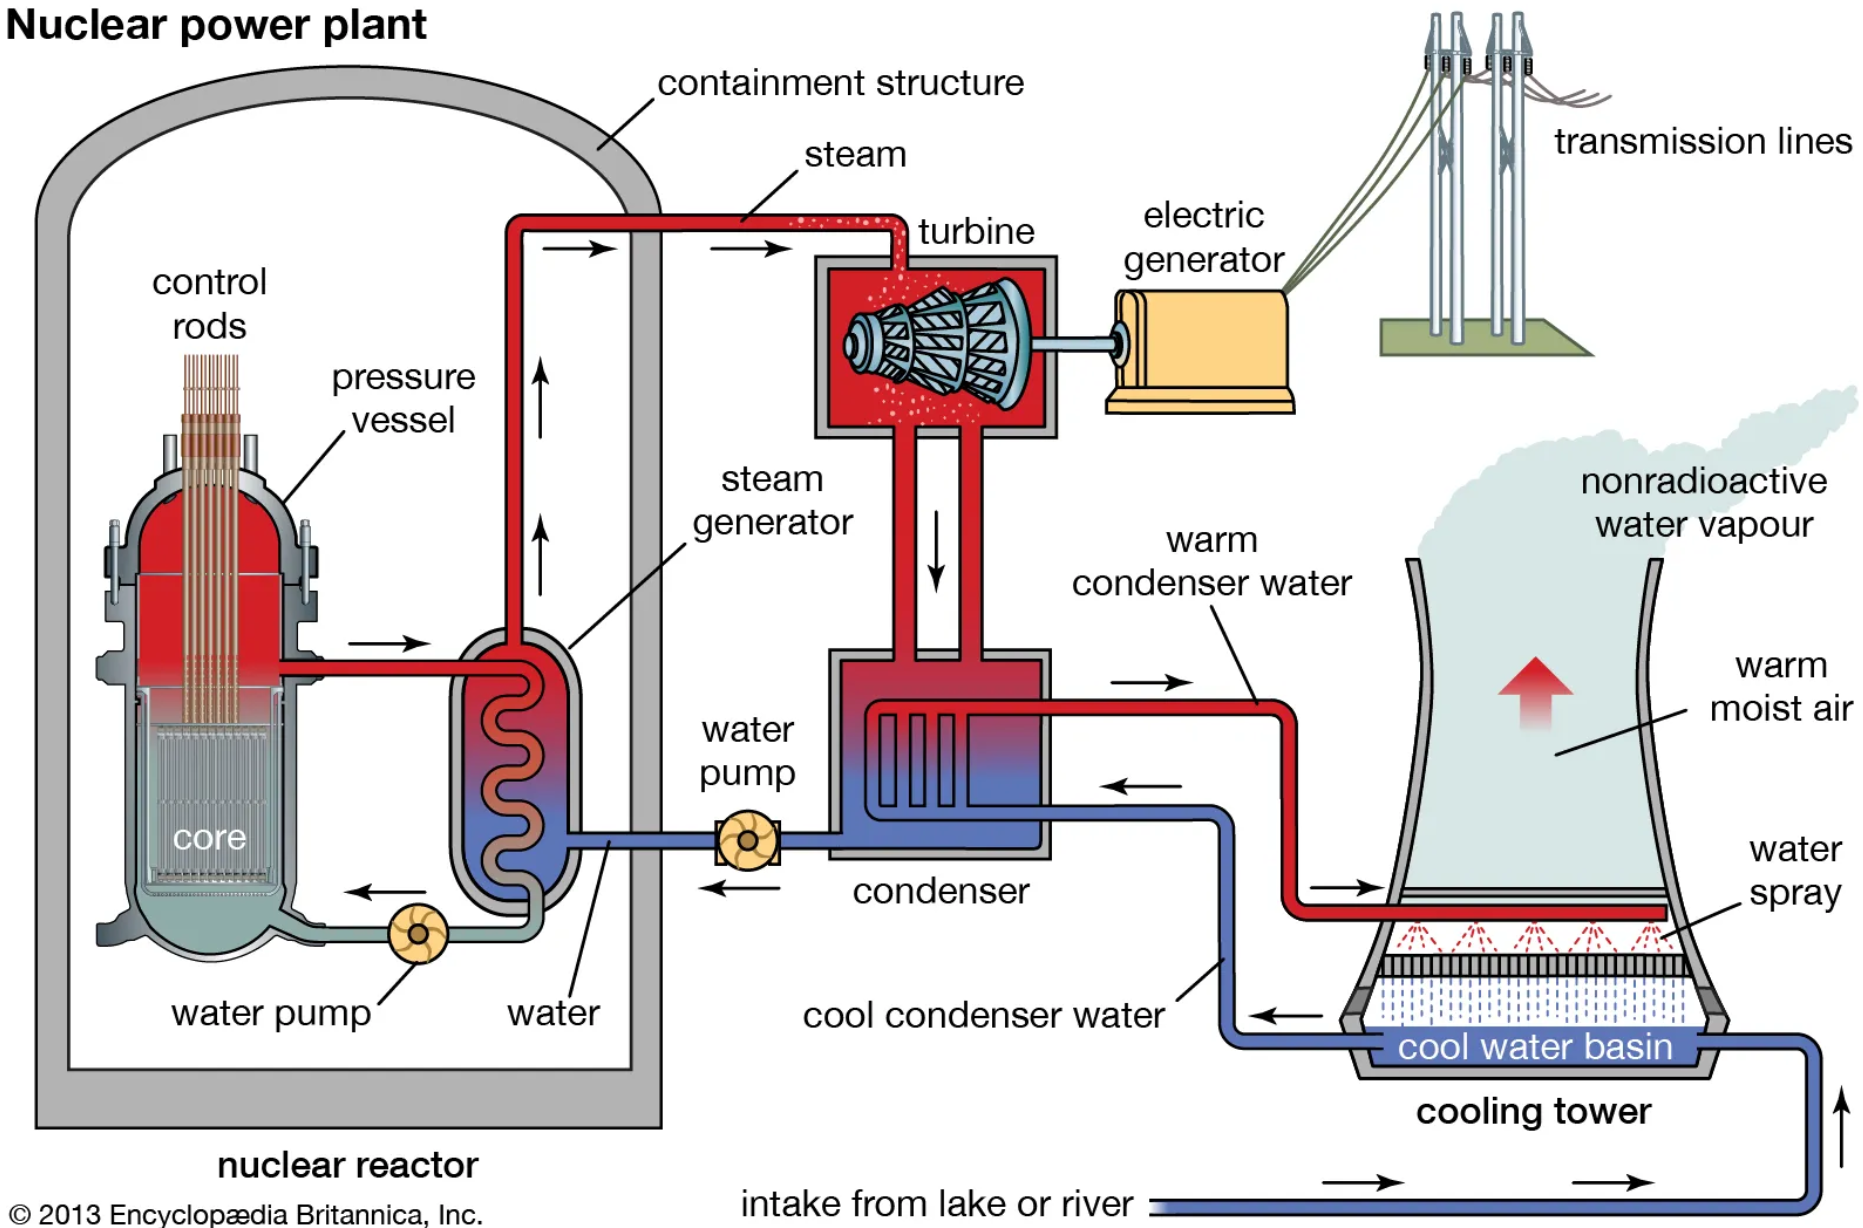
\includegraphics[width=\linewidth]{nuclear_plant}
  \end{center}
\end{frame}

\begin{frame}{Halogens}
  \begin{itemize}
  \item Fairly toxic and form acids when combined with
    hydrogen
  \item Readily react with metals to form salts e.g.
    NaCl
  \item Important for drug development due to their ``sticky''
    nature
  \item Prefers to gain an electron
  \end{itemize}
\end{frame}

\begin{frame}{My Research Project: Chlorolissoclimide}
  \begin{center}
    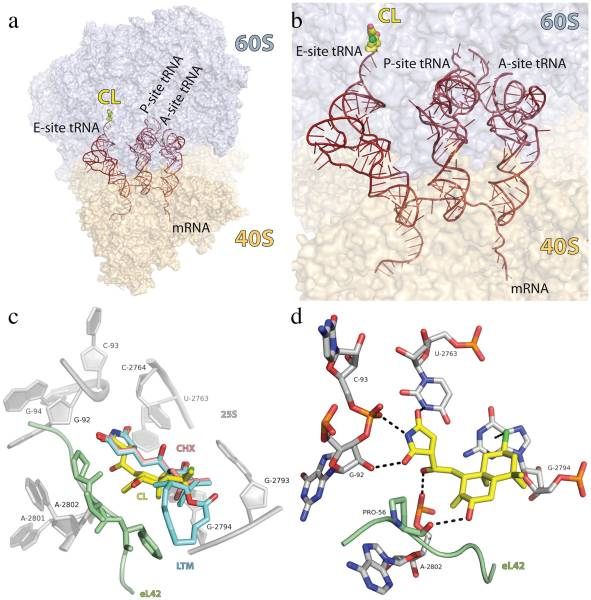
\includegraphics[trim={0 4.2in 0 0},clip,scale=0.45]{lisso_drug}
  \end{center}

  \begin{itemize}
  \item Chlorolissoclimide is a potent cancer drug that
    is naturally found in sea squirts
  \item Reference - doi: 10.1038/nchem.2800
  \end{itemize}
\end{frame}

\begin{frame}{Noble Gases}
  \begin{center}
    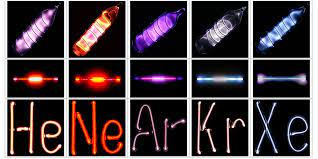
\includegraphics[scale=0.7]{neon_lights}
  \end{center}
  
  \begin{itemize}
  \item Colorless, odorless, tasteless, and non-flammable
    under standard conditions
  \item Extremely non-reactive and most stable elements
  \item Do not like to gain or lose electrons
  \end{itemize}
\end{frame}

\begin{frame}{Practice: Periodic Table}
  Group the elements into the following groups
  \begin{itemize}
  \item Br
  \item K
  \item Mg
  \item Al
  \item Mn
  \item Ar
  \item U
  \end{itemize}
\end{frame}

\begin{frame}{Practice}
  What is the charge of the ions for each of the following elements?

  \begin{itemize}
  \item Al
  \item P
  \item Br
  \item S
  \end{itemize}
\end{frame}

\end{document}
